\documentclass[a4paper]{article}
\renewcommand{\baselinestretch}{1.1}
\usepackage[utf8]{inputenc}
\usepackage[english]{babel}
\usepackage[T1]{fontenc}
\usepackage{graphicx}
\usepackage{hyperref}
\hypersetup{
	colorlinks = true,	
}
\usepackage{prettyref}
\newrefformat{fig}{A.\ref{#1}}
\usepackage{amsmath}
\usepackage{amssymb}
\usepackage{caption}
\usepackage[output-decimal-marker={,}]{siunitx}
\usepackage{booktabs}
\usepackage{subfig}
\usepackage{float}
\usepackage{geometry}
\usepackage{multicol}
\usepackage{listings}
\newenvironment{Figure}
	{\par\medskip\noindent\minipage{\linewidth}}
	{\endminipage\par\medskip}
\geometry{
	a4paper,
	total={170mm,257mm},
	left=20mm,
	top=20mm,
}

\title{Stellar Field Reconstruction}
\author{Alessandro Lattanzi}
\date{\today}

\begin{document}
	\maketitle
	
	\section{Introduction}
	The goal of this analysis is to implement an image reconstruction algorithm and check the properties of the reconstructed image. To this end a stellar field is first synthesized, the field is then "dirtied" in different ways and finally reconstructed using a Richardson-Lucy (henceforth referred to as RL) algorithm. A reconstruction using Gaussian fits is also run as a benchmark for the RL algorithm.\\
	The RL reconstruction works well in the center of the image and is gradually worse moving towards the borders. Some effects can appear in the image if the border isn't treated carefully and if the parameters for the superimposed PSF are not precise enough.\\
	\newline
	\textit{The full commented code and source material is available at \url{https://github.com/alelatt/Osservativa}}
	
	\vspace{0.035\textheight}
	\section{Metodology}
	\begin{multicols}{2}
		\subsection{Creation of a field}
			Having chosen a number of stars (N) to create and the image dimension in px, N sets (x, y, M) are extracted. The position coordinates (x, y) are taken from a uniform distribution with values in the range [0, image$\_$dim] and the mass, expressed in $M_{\odot}$, from a Salpeter distribution $N(M) = \frac{\alpha - 1}{M_0}(\frac{M}{M_0})^{-\alpha}$ with $\alpha = 2.35$, $M_0 = 0.4 M_{\odot}$, and values in the range $[0.4, 5] M_{\odot}$. The minimum is enforced by the function used for the generation (numpy.random.pareto) whereas the maximum is enforced by extracting a new mass if one is over $5M_{\odot}$.\\
			The mass range has been chosen arbitrarily in order to ensure that the Salpeter distribution is a sensible choice and in order to avoid stars too bright that would overshadow any attempt at visualizing the image.\\
			The mass is then converted to luminosity (in $L_{\odot}$) using:
			\[
				\begin{array}{lc}
					L = M^4 & \text{for } M\in[0.4,2]M_{\odot}\\
					L = 1.4 \cdot M^{1.5} & \text{for } M>2M_{\odot}
				\end{array}
			\]
			\newline
			\underline{\textbf{NB:}} The conversion formula for $M>2M_{\odot}$ used is\\ 
			\indent\indent wrong. The correct conversion is $L = 1.4 \cdot M^{3.5}$.\\
			\indent\indent This souldn't affect the results of the\\
			\indent\indent reconstruction, it just changes the initial\\
			\indent\indent luminosity distribution.\\
			
			The luminosity values are then converted to a pixel readout value by setting a reading of 10 for a $0.4M_{\odot}$ star. This last step was used to have a reference luminosity to compare to the background luminosity, which will be used later.\\
			
			The procedure used up to here is what is needed to create the "true" field.\\
			
			The "observed" field is then obtained by adding one or more effects to the "true" field. The reconstruction was run on fields convoluted with a Gaussian PSF without background, with background, and with Poisson noise (and no background)\footnote{The order of operations used is: "true" field $\rightarrow$ background $\rightarrow$ convolution with Gaussian PSF $\rightarrow$ Poisson noise}.\\
			
		\subsection{Finding background and PSF width}
			It's assumed that the PSF is a Guassian and that it's the same for the whole field.\\
			
			The parameters needed for the reconstruction are the Gaussian PSF's sigma and the background intensity (offset). These parameters are found by fitting some of the brightest stars in the image.\\
			A 1D Gaussian is fitted onto the minimum profile around the brightest pixel. This "minimum profile" is the profile obtained by taking the faintest pixel at each distance around the peak. This is done in order to minimize the effects that an overlap with other stars may have.\\
			The obtained parameters (which include the brightness of the underlying star) are used to compute a 2D board that reproduces the fitted star and extends up to $4\sigma$ in all directions and is used to "remove" the brightest star from the image.\\
			This process is repeated as many times as wanted and the final sigma and PSF width are given as the weighted averages over all the fitted stars.\\
			
			Since the assumption is that only a Gaussian PSF and some background luminosity are added, this fitting method becomes less precise as soon as any form of noise is added.\\
			
		\subsection{Reconstruction using RL}
			The field is then reconstructed using the RL algorithm, an iterative process based on Bayes' theorem.\\
			
			The width of the PSF found in the first step is used to compute a board which contains the PSF up to $4\sigma$ in all directions, needed in the reconstruction.\\
			
			First it's worth noting that a constant background can in principle be removed before starting the reconstruction. If the image before convolving with the PSF is $i$(x,y), we can write $i(x,y) = c(x,y) + b$ where $c$(x,y) is the background-subtracted image and $b$, a matrix of constant value, is the background.
			Letting $o$(x,y) be the observed image and $g$(x,y) the PSF, and assuming that the background is constant, we can write, omitting the coordinates, $o = i \otimes g = (c \otimes g) + (b \otimes g)$, but, since g is normalized and b is constant, this reduces to $o = (c \otimes g) + b$. We thus run the reconstruction on $c$(x,y) by subtracting the background before any other operation on the image.\\
			\newline
			
			Letting $f_i$(x,y) be the reconstructed image at the i-th iteration, then:
			\begin{equation*}
				f_{i+1} = \left\{\left[\frac{c}{f_i \otimes g}\right] \otimes g^T\right\}f_i
			\end{equation*}
			This algorithm needs a starting condition $f_0$ from which the iteration can begin. The observed image (background-corrected) is used as $f_0$.\\
			
			The algorithm is considered done when a set number of iterations is completed or if the last minimum in the $\chi^2 \doteq \sum_{x,y}\left\{c-\left[\left(f_{i+1} + b\right) \otimes g \right]\right\}^2$ was found more than a set number of steps before the current one.\\
			The returned image is the one with the lowest $\chi^2$ from the computed ones.
			
		\subsection{Reconstruction using Gaussian fit}
			As a benchmark for the RL reconstruction this method takes advantage of a similar technique as the one used to find the PSF and offset.\\
			
			The reconstruction starts from the brightest peak and fits the minimum profile, keeping sigma and offset constrained so as to fit only the amplitude of the Gaussian.\\
			The fitted amplitude is used to get the intensity of the star, taken as a delta centered in the peak. The star is then saved in an output image.\\
			A board is then constructed by convolving a Gaussian of the correct sigma to the reconstructed star as to get back the contribution of the star to the observed image. This board is then subtracted from the image in order to remove the signature of the star.\\
			The procedure then starts back by taking the new brightest peak.\\
			
			The end conditions are the same as for the RL reconstruction.\\
			
			The assumption behind this procedure is again that there's only a Gaussian PSF and an offset, so it's less precise when noise is added.
		
	
	\end{multicols}

	\vspace{0.035\textheight}

	\section{Results}
	\begin{multicols}{2}
		\subsection{General definitions and methods}
			The output images from both algorithms were analyzed in two aspects: luminosity distribution of the pixels and completeness of the sample.\\
			
			The completeness of the reconstruction is computed on a pixel-by-pixel basis by simulating 5000 images and combining the results. Completeness is defined here as the frequency in which a star is correctly reconstructed. A star is considered correctly reconstructed if the position on the reconstructed image matches that of the original image and if the luminosity is within a certain percentage of the original. Thus completeness also varies depending on the chosen precision in luminosity.\\
			
			The luminosity distribution was studied by plotting on a histogram the number of pixels per interval in luminosity.\\
		
	\end{multicols}
		\subsection{No Poisson noise}
		
			\begin{figure}[h!]
				\centering
				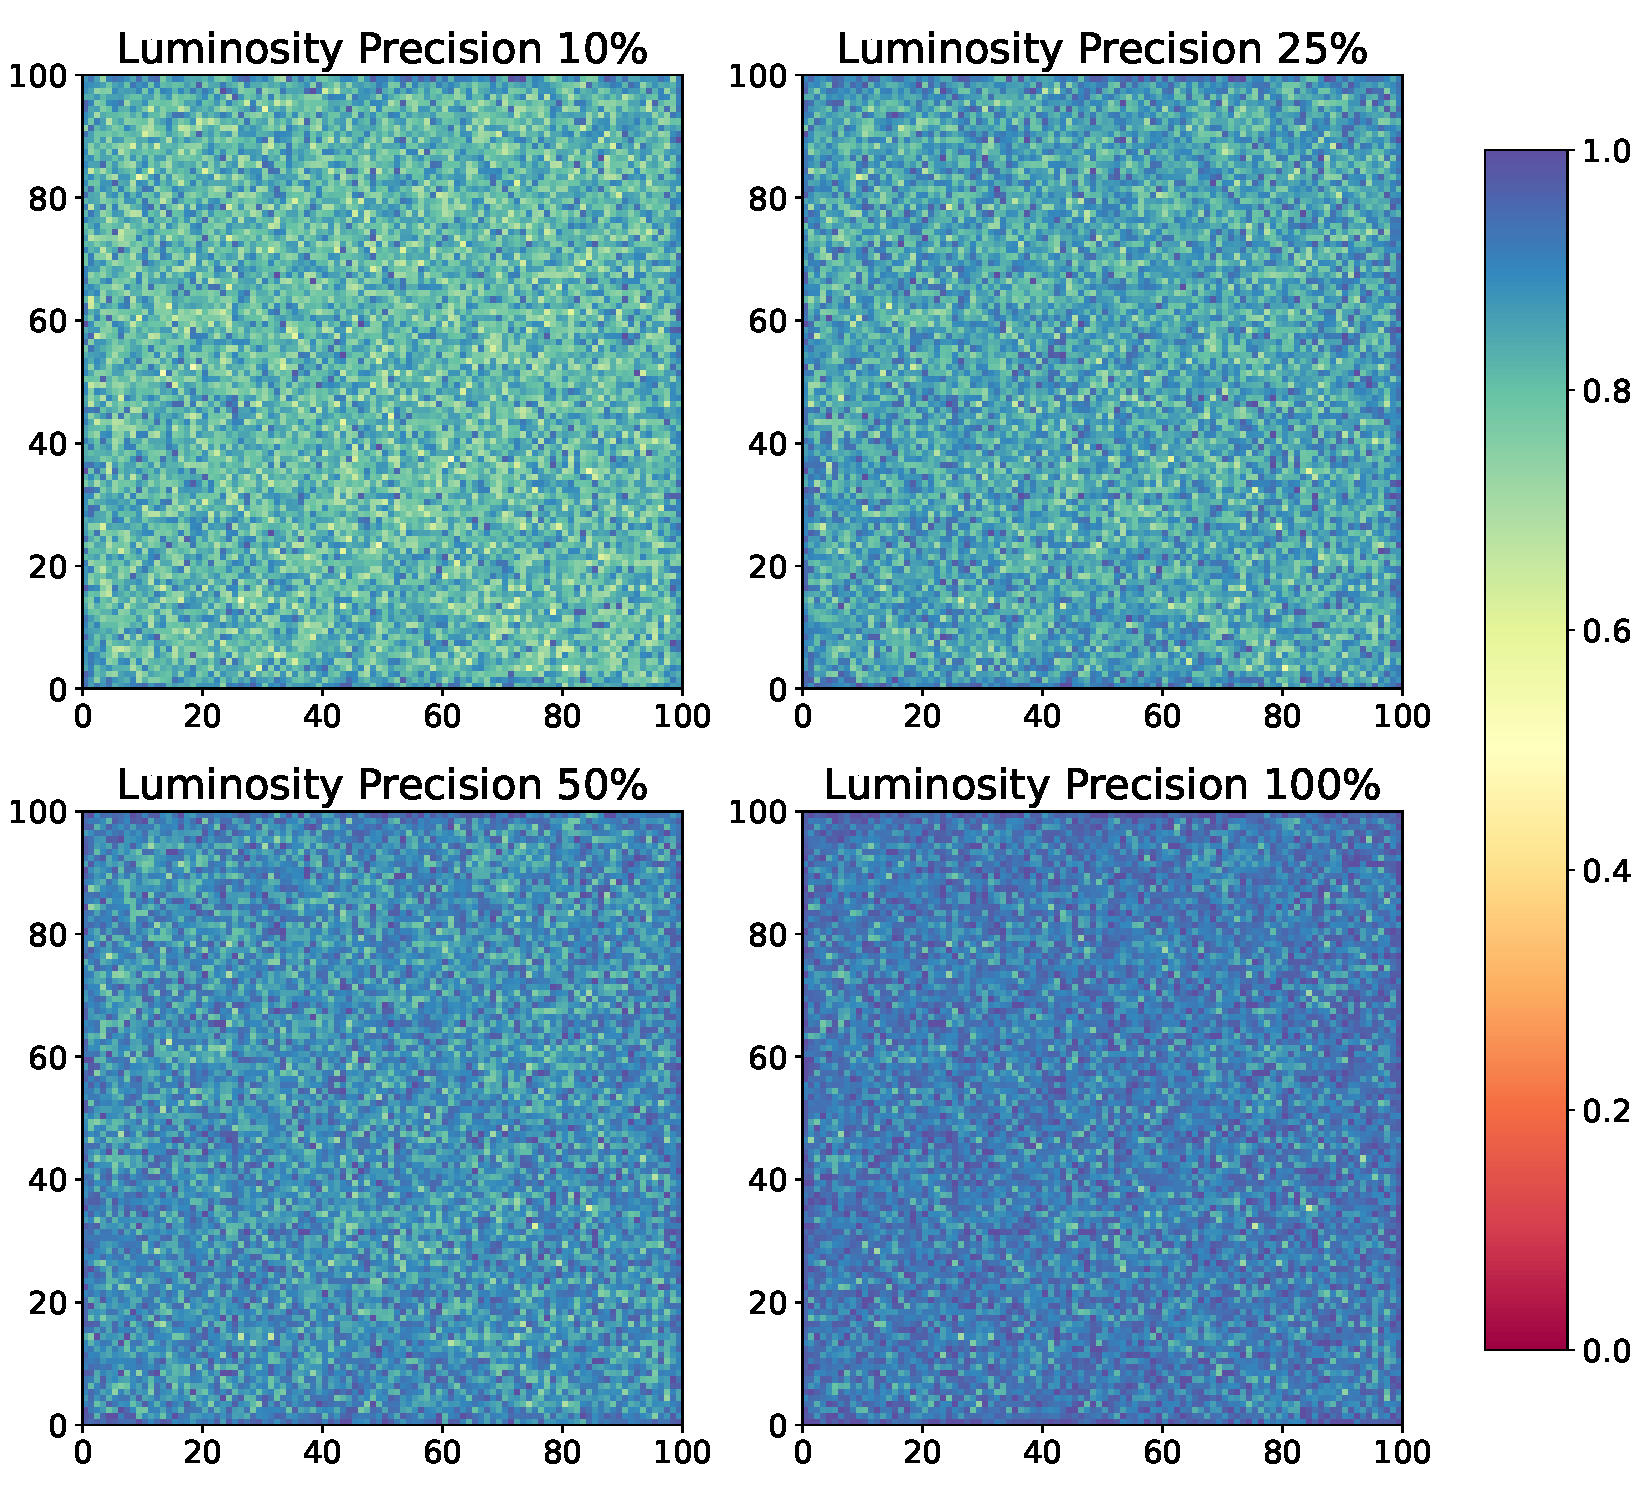
\includegraphics[width=0.6\linewidth]{gauss2_boards_gauss.pdf}
				\caption{Completeness of Gaussian fit at various luminosity precisions, $\sigma = 2$, off = 0}
				\label{fig:gbg}
			\end{figure}
			\begin{figure}[h!]
				\centering
				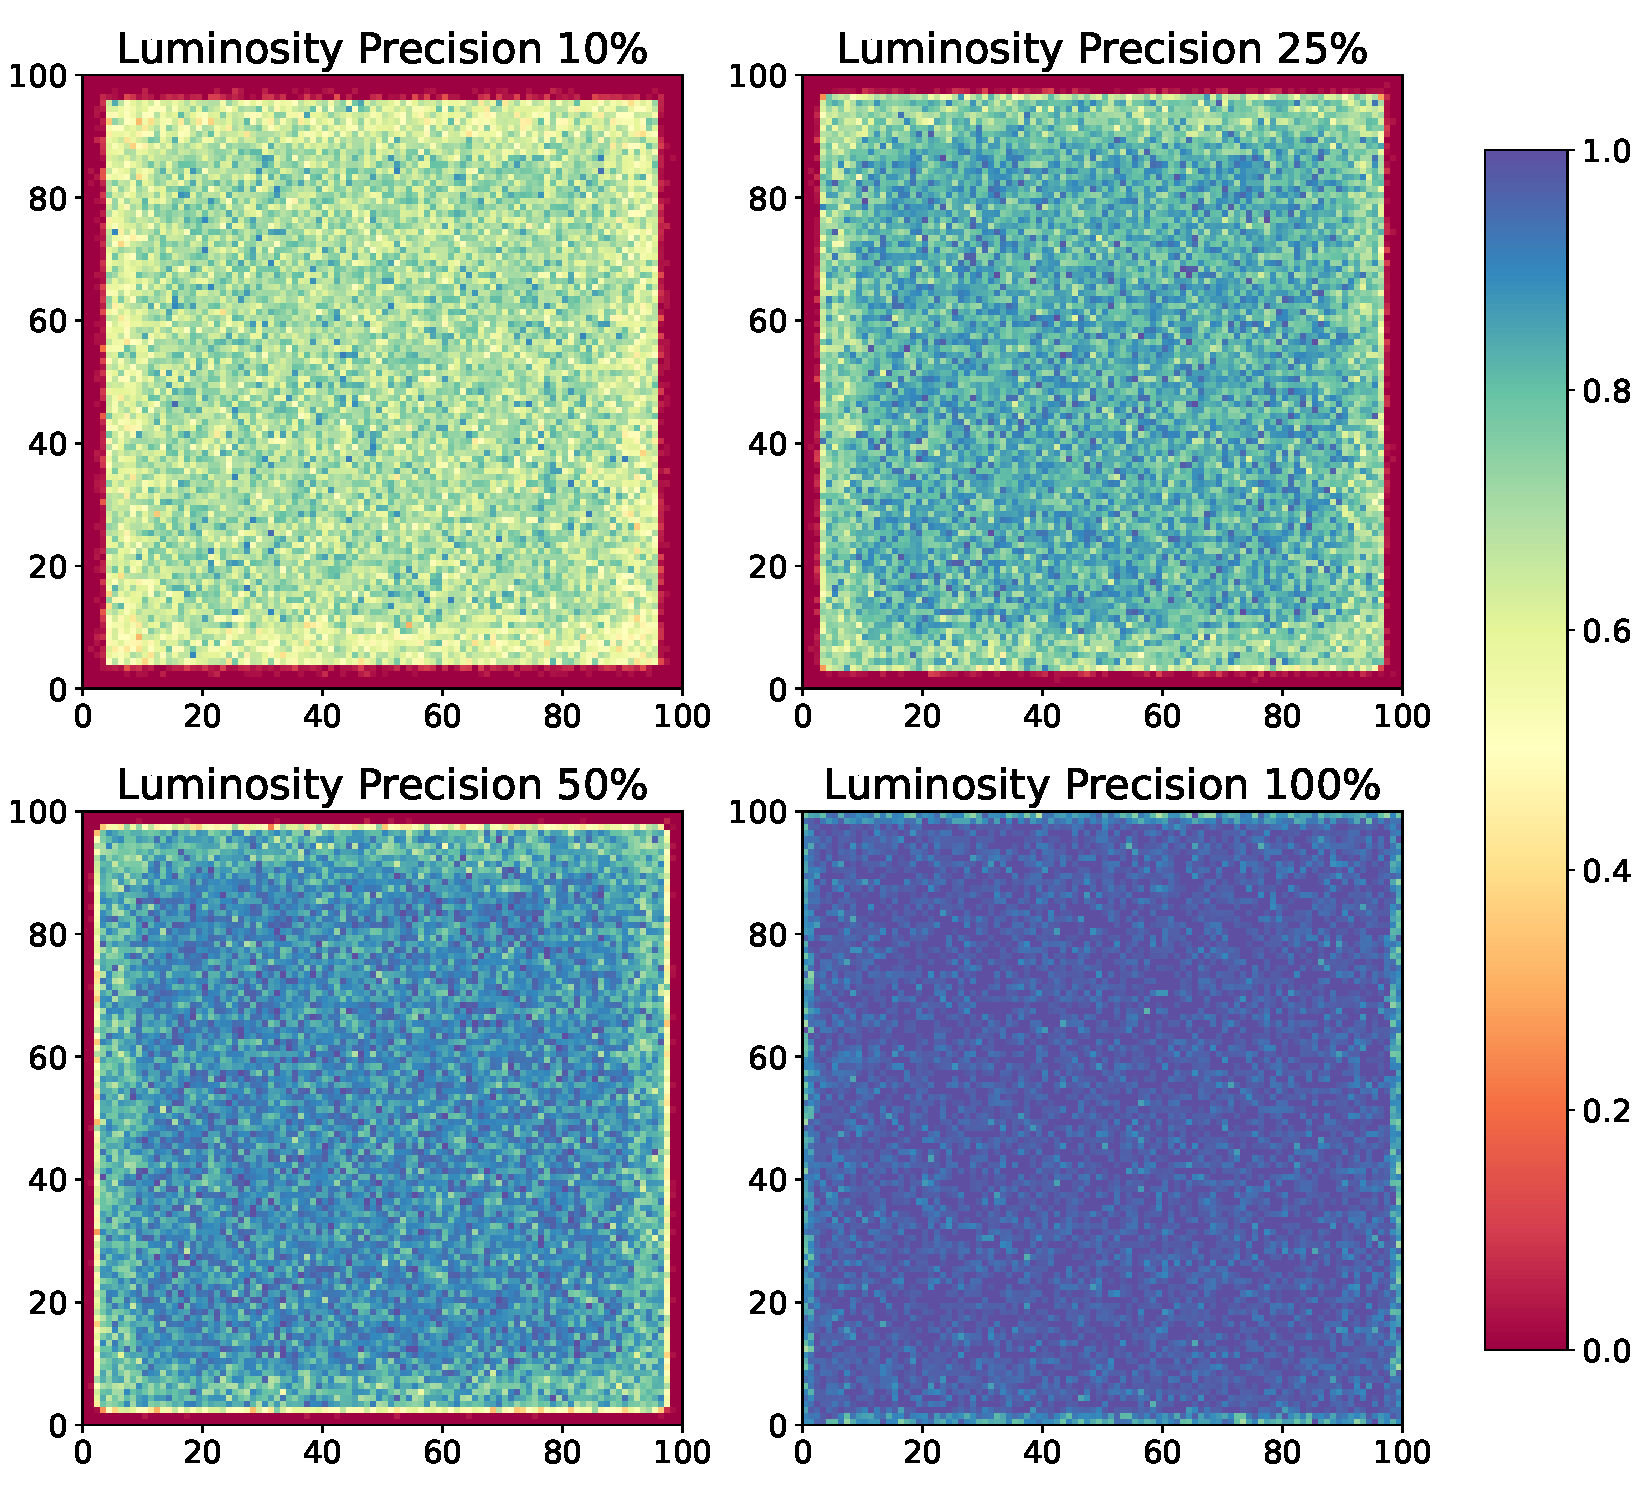
\includegraphics[width=0.6\linewidth]{gauss2_boards_lucy.pdf}
				\caption{Completeness of RL reconstruction at various luminosity precisions, $\sigma = 2$, off = 0}
				\label{fig:gbl}
			\end{figure}
	
	\begin{multicols}{2}
			When no Poisson noise is present RL gives better results in the middle of the image and at lower luminosity precision with respect to the Gaussian fit benchmark (Figure \ref{fig:gbg}, Figure \ref{fig:gbl}).\\
			
			The lower completeness of the RL algorithm near the borders is due to a shift inwards of the position of stars and a bad luminosity reading. Both of these effects are due to how the convolution works.\\
			
			By convolving with the PSF, the luminosity of stars near the border of the image is spread in part out of the image and is thus lost. Having removed the offset the only assumption that can be made is that outside the image's borders there's nothing.\\
			
			Since RL conserves flux, the intensity that can be reconstructed is limited by that inside the image, thus a lower luminosity for the reconstructed stars is to be expected and with it a lower completeness when choosing a higher precision in luminosity.\\
			This can also cause a shift of the stars near the border to the inside. Looking at a star after the convolution with a PSF, a bigger part of the total luminosity is now towards the center of the image with respect to the brightest point, since towards the border part of it fell outside and was lost. This can be reconstructed as a star shifted to the inside.\\
			
			The Gaussian fit reconstruction is more uniform in its performance since in principle there only needs to be one point at each distance from the peak in order to fit, so the border only has a minimal effect. On the other hand many factors can influence the goodness of the fit, so this method is on average worse than RL.\\
			The better performance at higher luminosity precision (Figures \ref{fig:ghg} and \ref{fig:ghl}) is probably due to the fact that by fitting a star is identified in one step and, even if the fit isn't perfect, what's left is little relevant for subsequent fits. This characteristic is highlighted by the fact that the Gaussian reconstruction often finishes before the maximum amount of steps is reached, since in few steps (comparable to the number of stars present) the $\chi^2$ reaches a minimum (having fitted all the stars) and starts going back up, thus stopping the algorithm.\\
			
			Since the background is removed before the RL reconstruction and is a fixed parameter in the Gaussian reconstruction, little to no difference can be seen between having background or not (Figures \ref{fig:gbg} - \ref{fig:ghl} and figures \ref{fig:bbg} - \ref{fig:bhl}), and what little can be seen is probably due to slight differences in the efficiency of the initial determination of sigma and offset.\\
			\newline
			\newline
			\underline{\textbf{NB:}} Due to the mistake in the luminosity\\
			\indent\indent conversion, the discontinuity in the distribution\\
			\indent\indent corresponds to $L(M \rightarrow 2M_{\odot}^+)$, the upper limit\\
			\indent\indent corresponds to $L(M \rightarrow 2M_{\odot}^-)$\\
			
			\begin{Figure}
				\centering
				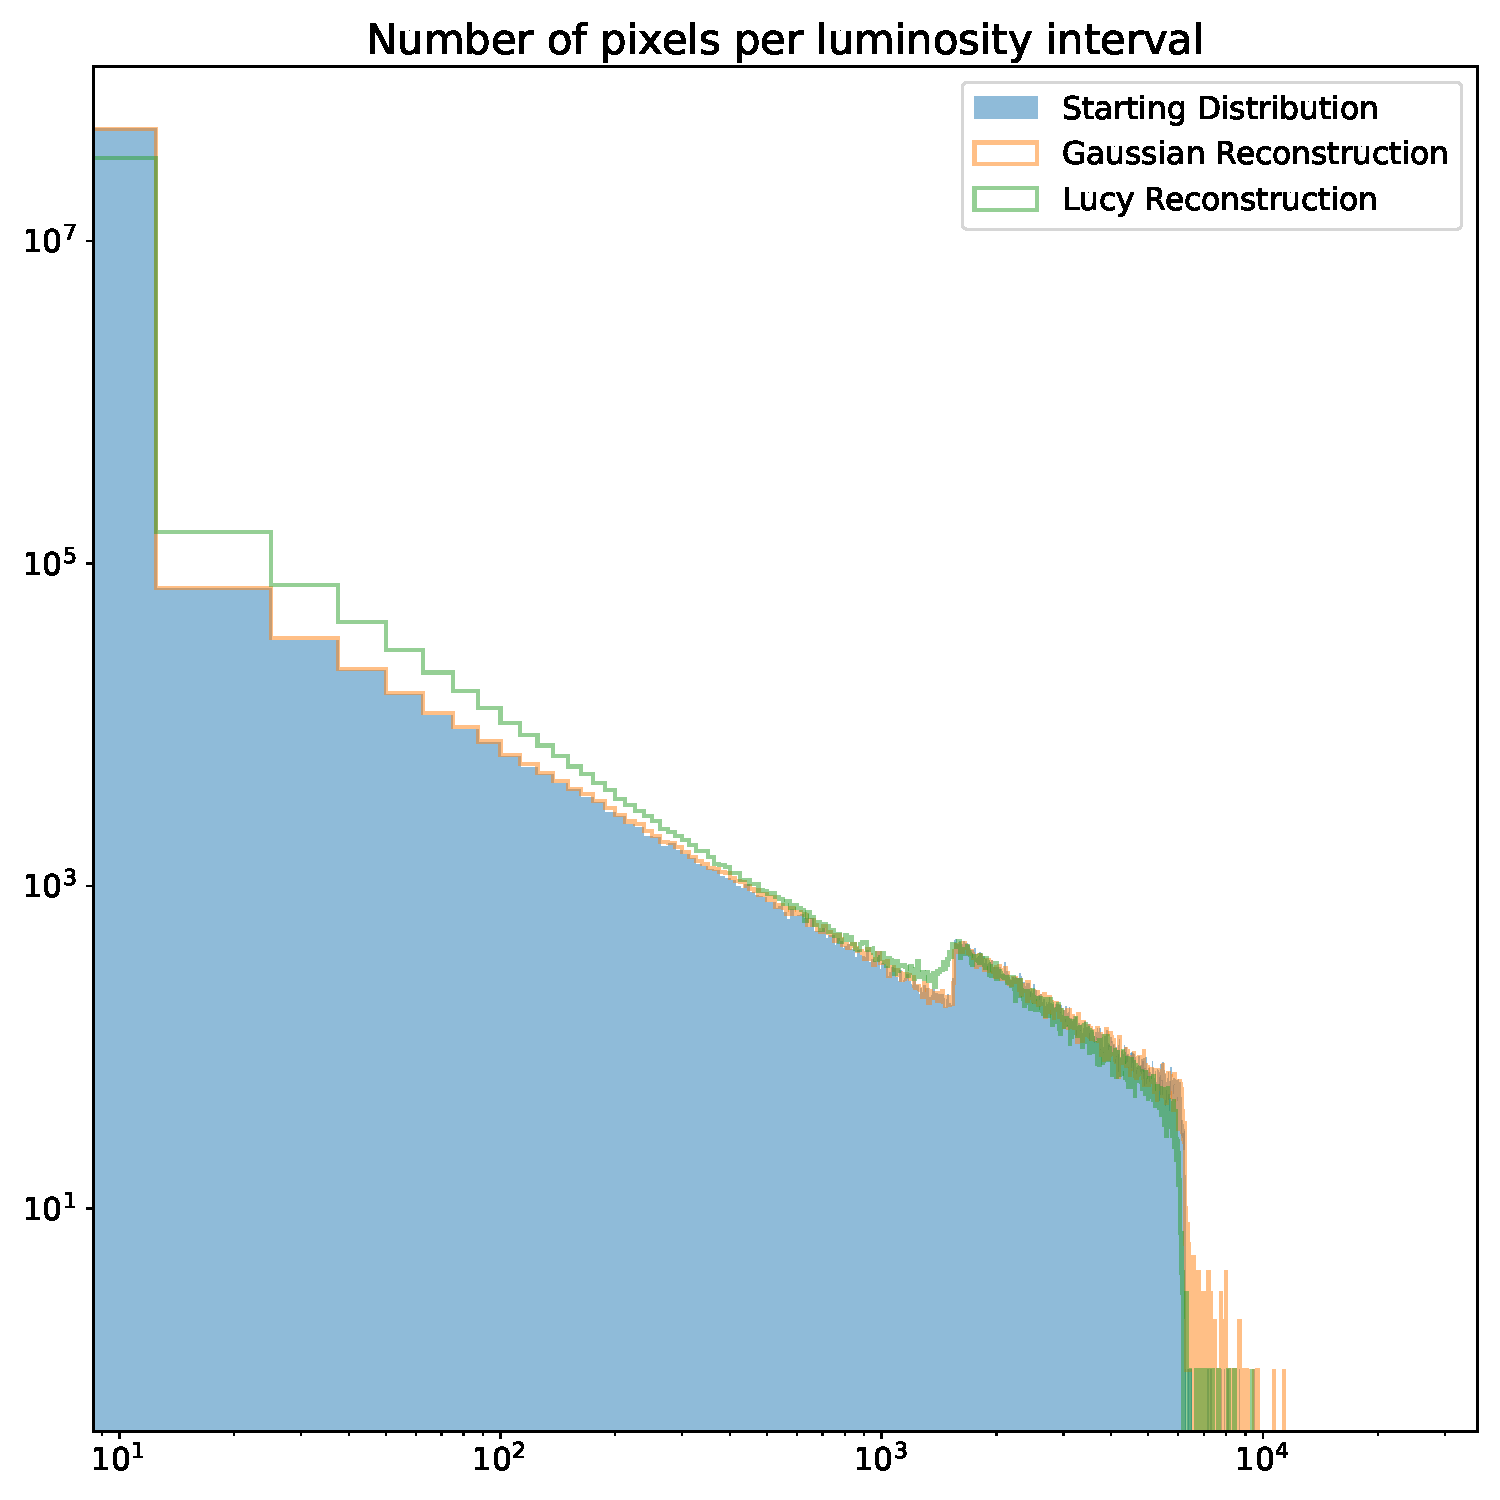
\includegraphics[width=\linewidth]{gauss2_lumin.pdf}
				\captionof{figure}{Luminosity distribution, $\sigma = 2$, off = 0}
				\label{fig:gl}
			\end{Figure}
			
			The luminosity distribution of the Gaussian reconstruction more closely matches the original one, with notable exceptions at high luminosities.\\
			
			The luminosity distribution of the RL reconstruction is closer to the original at high luminosity, it reconstructs less very bright and very faint pixels and, most notably, reconstructs more mid-to-low luminosity pixels. These mistakes in the reconstruction are due to the initial fit, that gives a good, but not perfect, estimate of sigma and offset. These ever so slightly wrong parameters cause a "smearing" of the luminosity in the reconstructed image, thus explaining both the relative lack of very faint and very bright pixels and an abbundance of low-to-mid luminosity pixels.\\
			
			As expected there is little difference in the luminosity distributions between background (Figure \ref{fig:bl}) and no background (Figure \ref{fig:gl}).\\
			
			In general it's also worth noting that the total luminosity contained in the images reconstructed with RL is, on average, $\sim 3.5\%$ less than the original. Since the RL algorithm conserves flux, this can give an estimate of how much light is lost outside the image when applying the PSF.
		
		\newpage
		\subsection{Poisson noise}
			The first crucial aspect when adding Poisson noise is that the initial Gaussian-fit based procedure to find sigma and offset is very imprecise, thus the following reconstructions suffer greatly by a poor estimation of these parameters.\\
			
			Adding Poisson noise after the Gaussian PSF the RL algorithm is definitely better than the Gaussian fit (Figures \ref{fig:pbg} - \ref{fig:phl}). This is to be expected, since the Gaussian fit algorithm has no way to mitigate the effect added by the noise.\\
			It's also worth noting that the Gaussian fit is still uniform across the image in its performance and the RL still has border effects.\\
			
			Looking at the luminosity distributions (Figure \ref{fig:pl}) it's clear that the previously identified effects for both methods are here exaggerated.\\
			
			The Gaussian fit reconstructs well mid-to-high luminosity pixels, where the added noise is small compared to the original luminosity and also reconstructs well near zero luminosity, where the added noise is near to zero. In the mid-luminosity region there's a shift to higher luminosities given by the additive noise.\\
			
			The RL reconstruction still shows the results of "smearing", having less near-zero luminosity pixels, less very bright pixels and more low-to-mid luminosity pixels.	
	\end{multicols}

	\vspace{0.035\textheight}

	\section{Final Remarks}
		Overall the RL algorithm demonstrates an excellent ability at reconstruction, especially when adding noise.\\
		
		Some additional performance could be recovered by finding a more precise way to fit the initial parameters sigma and offset. This could be achieved through a semiblind RL reconstruction (in which both the image and the PSF need to be recovered, but the analytical form of the PSF is known). This additional performance could greatly improve the reconstruction with Poisson noise (since it was negatively impacted by a bad initial parameter estimation). The no-noise reconstruction could also benefit from a better estimate of the initial parameters, especially the offset, which was noted as being a delicate parameter in the reconstruction.\\
		
	\newpage
	\section{Referenced figures}
		\begin{figure}[h!]
			\centering
			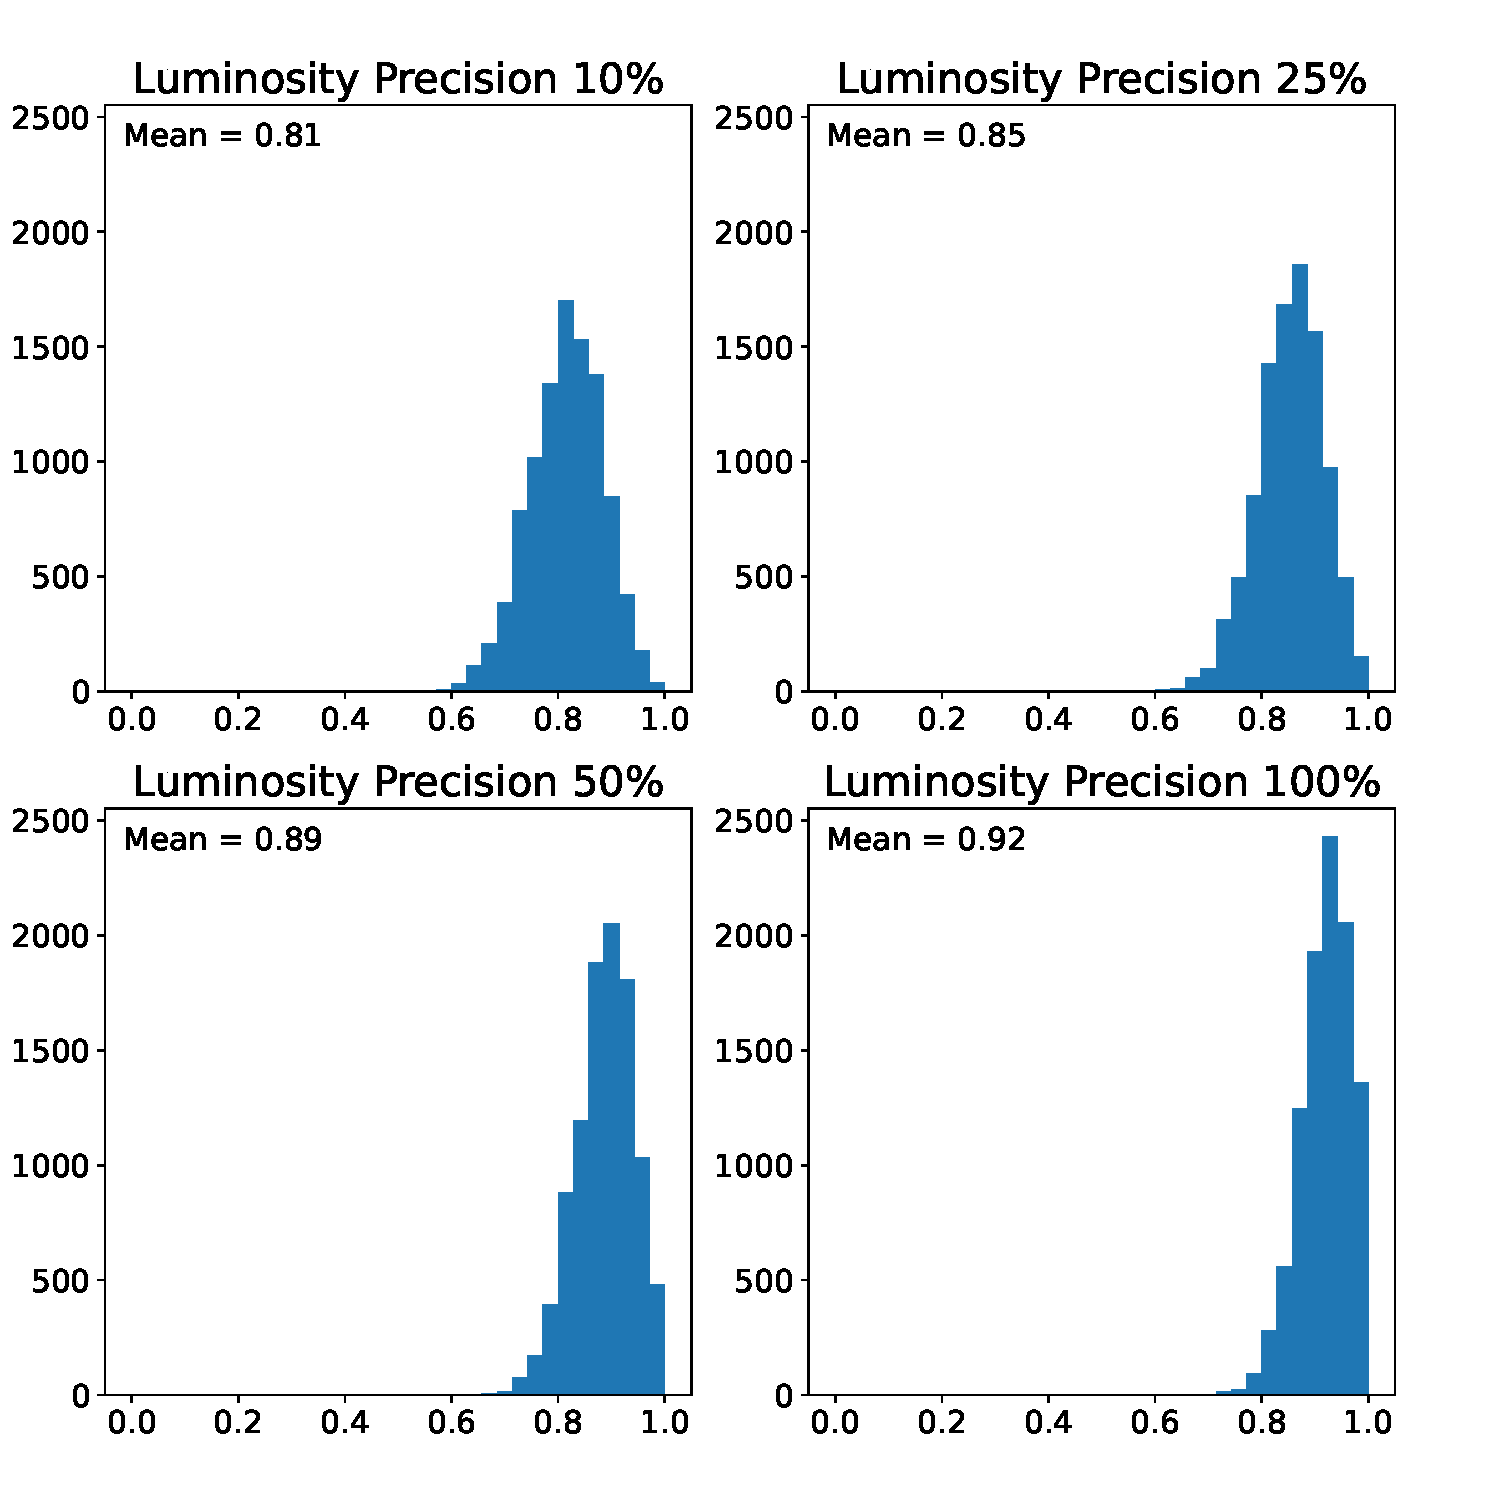
\includegraphics[height=0.4\textheight]{gauss2_hists_gauss.pdf}
			\caption{Completeness distribution of Gaussian fit, $\sigma = 2$, off = 0}
			\label{fig:ghg}
		\end{figure}
		\begin{figure}[h!]
			\centering
			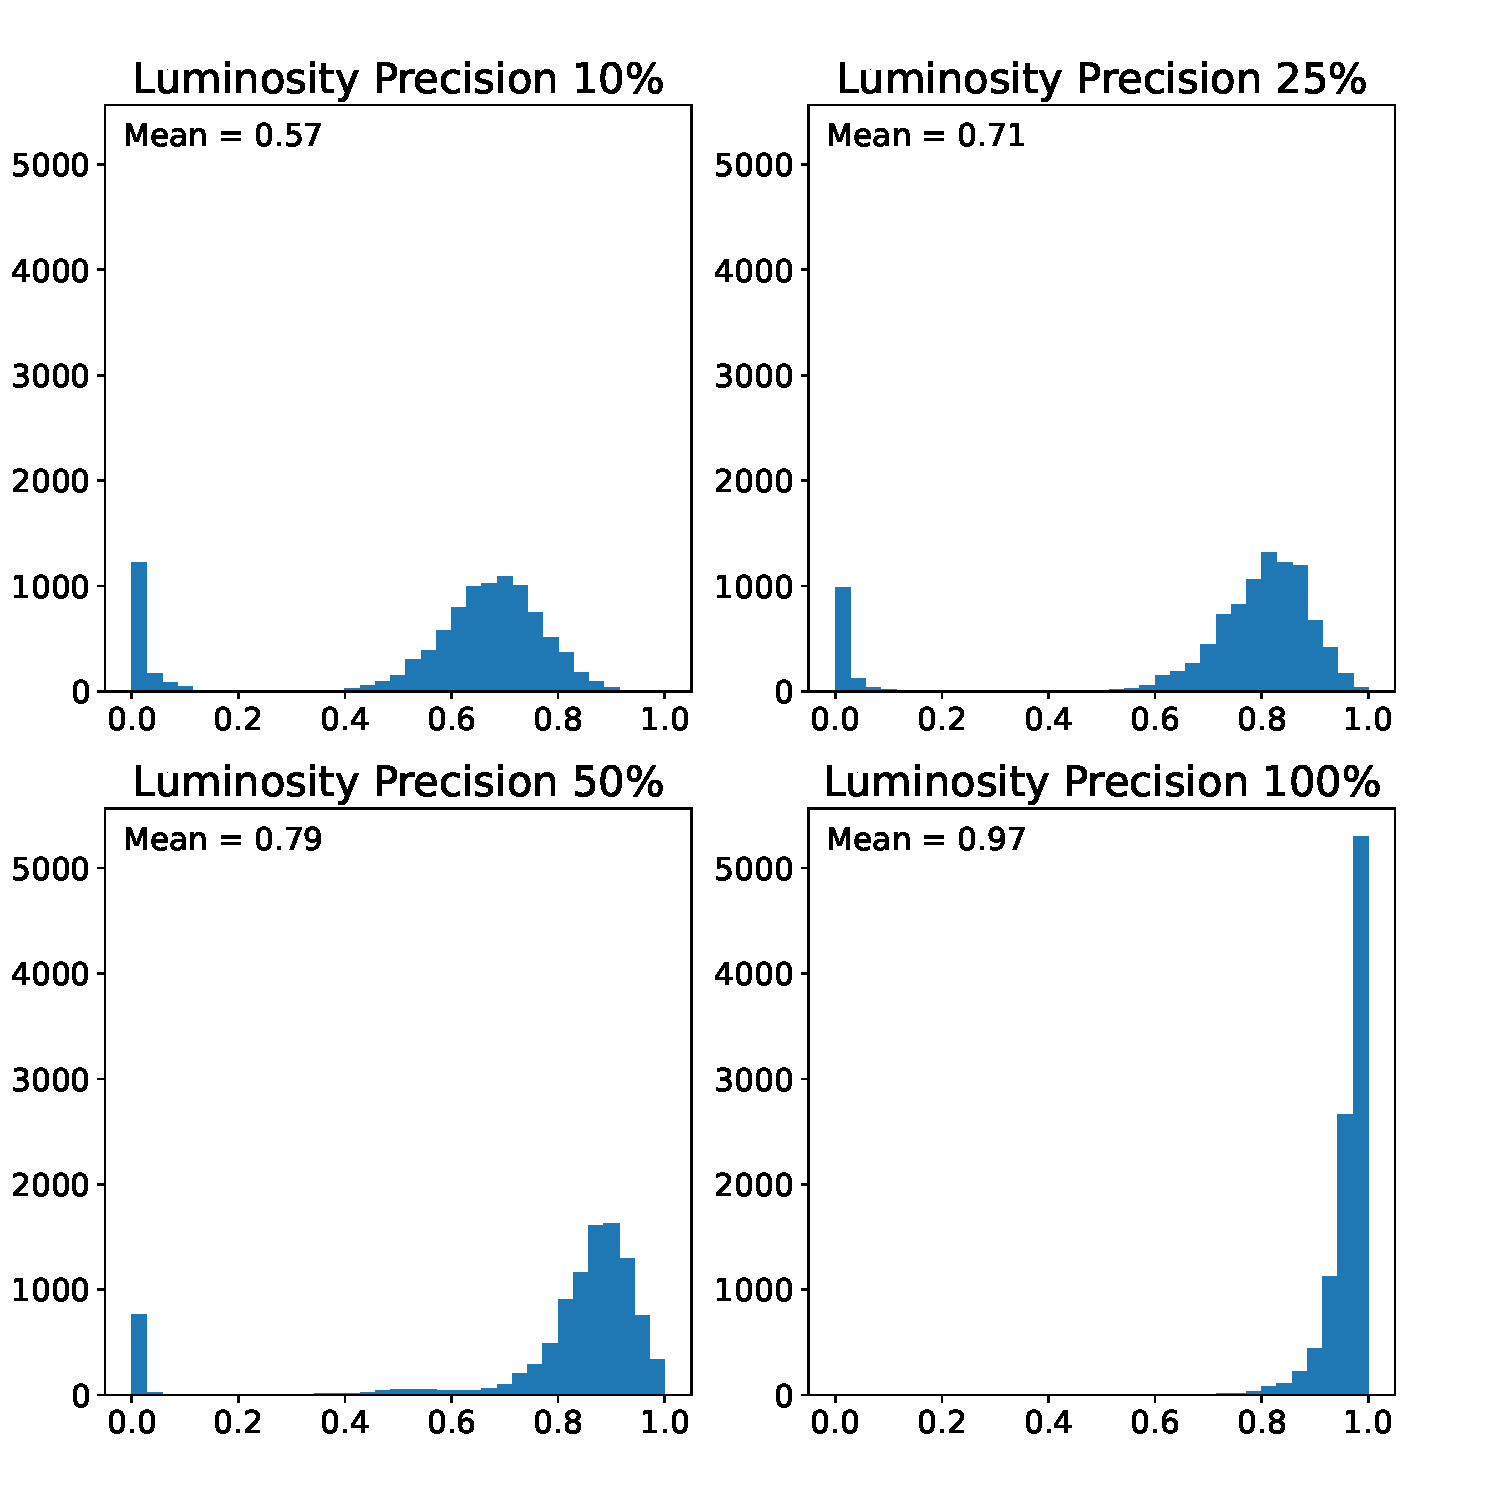
\includegraphics[height=0.4\textheight]{gauss2_hists_lucy.pdf}
			\caption{Completeness distribution of RL reconstruction, $\sigma = 2$, off = 0}
			\label{fig:ghl}
		\end{figure}
		\newpage
		\begin{figure}[h!]
			\centering
			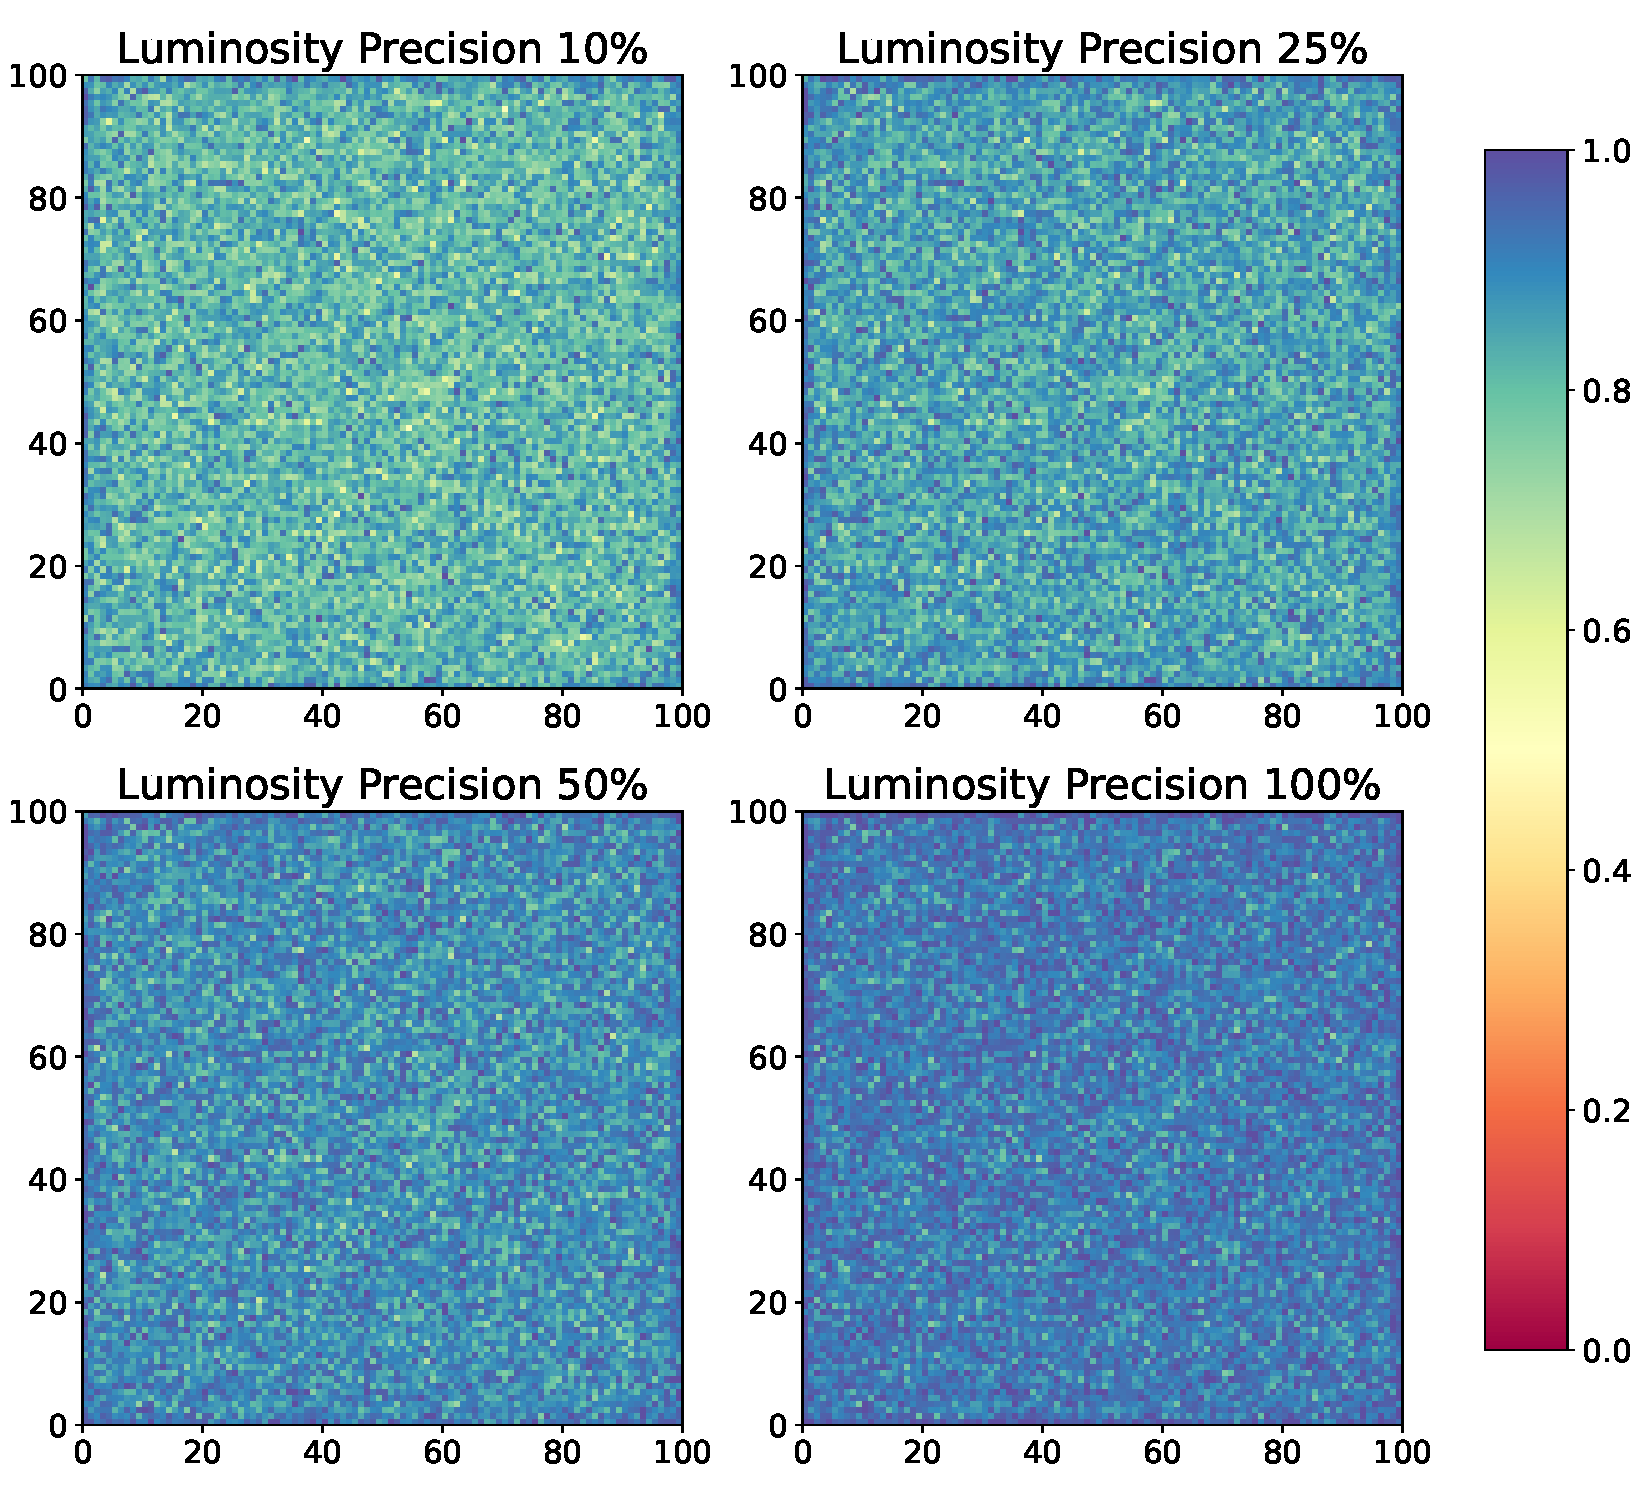
\includegraphics[height=0.4\textheight]{backgauss2_boards_gauss.pdf}
			\caption{Completeness of Gaussian fit, $\sigma = 2$, off = 10}
			\label{fig:bbg}
		\end{figure}
		\begin{figure}[h!]
			\centering
			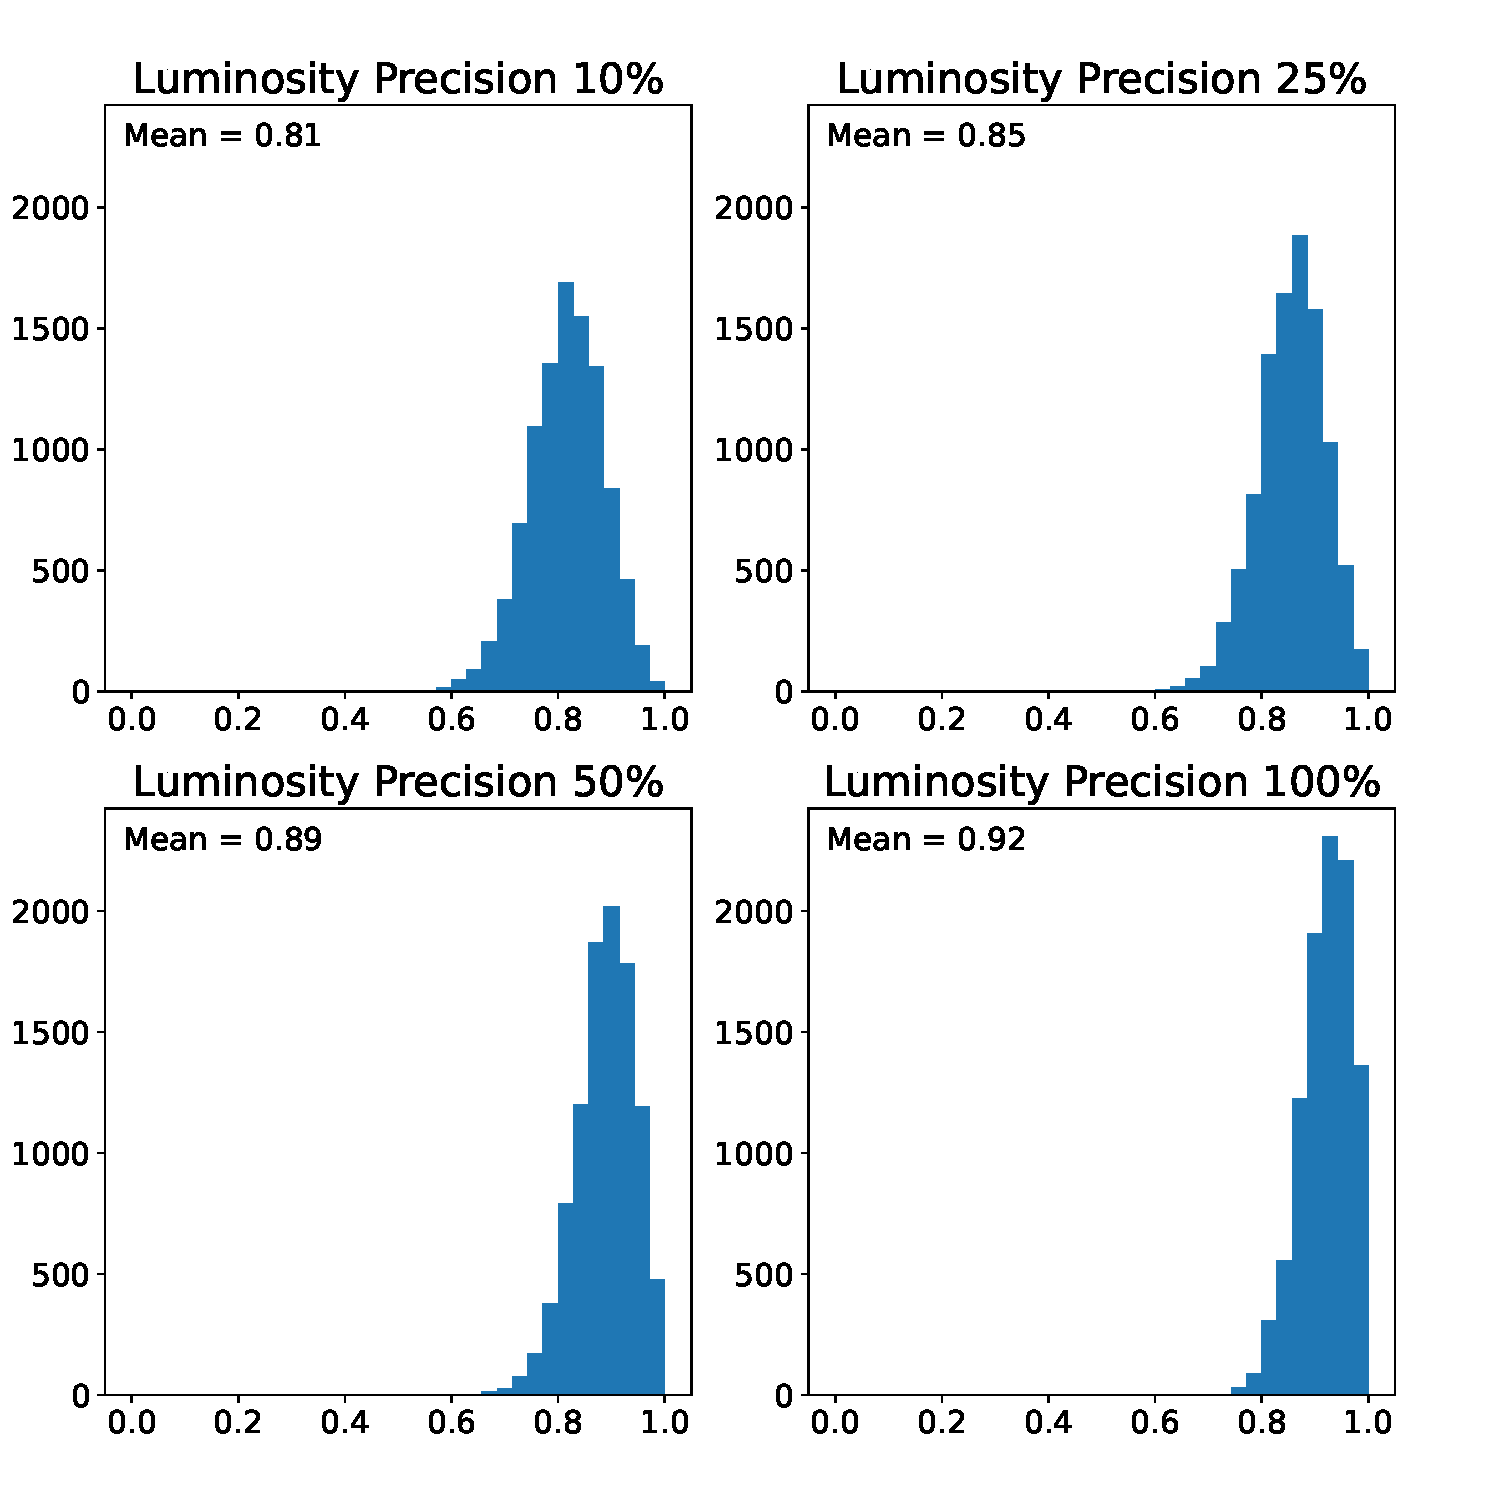
\includegraphics[height=0.4\textheight]{backgauss2_hists_gauss.pdf}
			\caption{Completeness distribution of Gaussian fit, $\sigma = 2$, off = 10}
			\label{fig:bhg}
		\end{figure}
		\newpage
		\begin{figure}[h!]
			\centering
			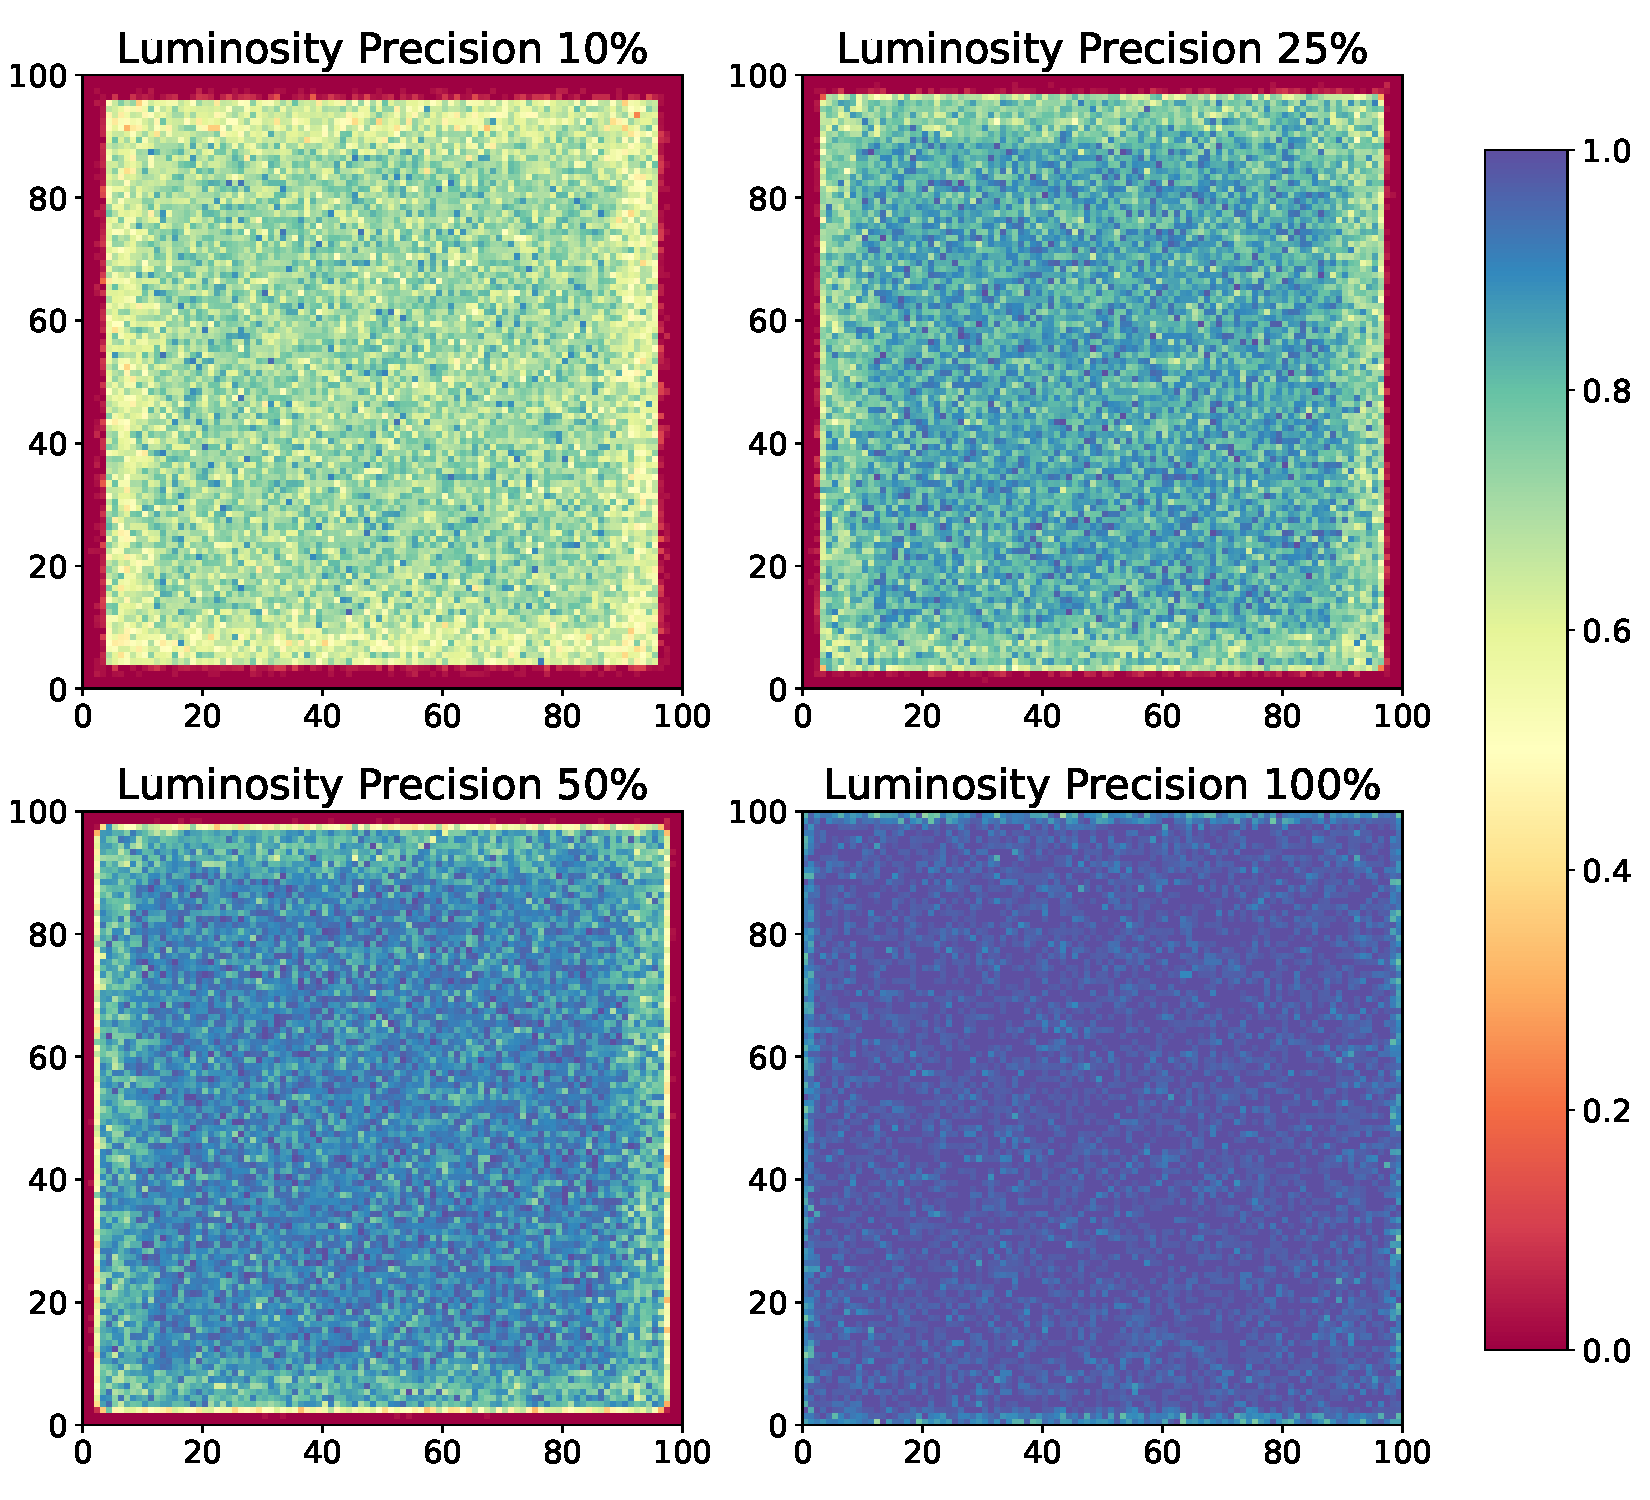
\includegraphics[height=0.4\textheight]{backgauss2_boards_lucy.pdf}
			\caption{Completeness of RL reconstruction, $\sigma = 2$, off = 10}
			\label{fig:bbl}
		\end{figure}
		\begin{figure}[h!]
			\centering
			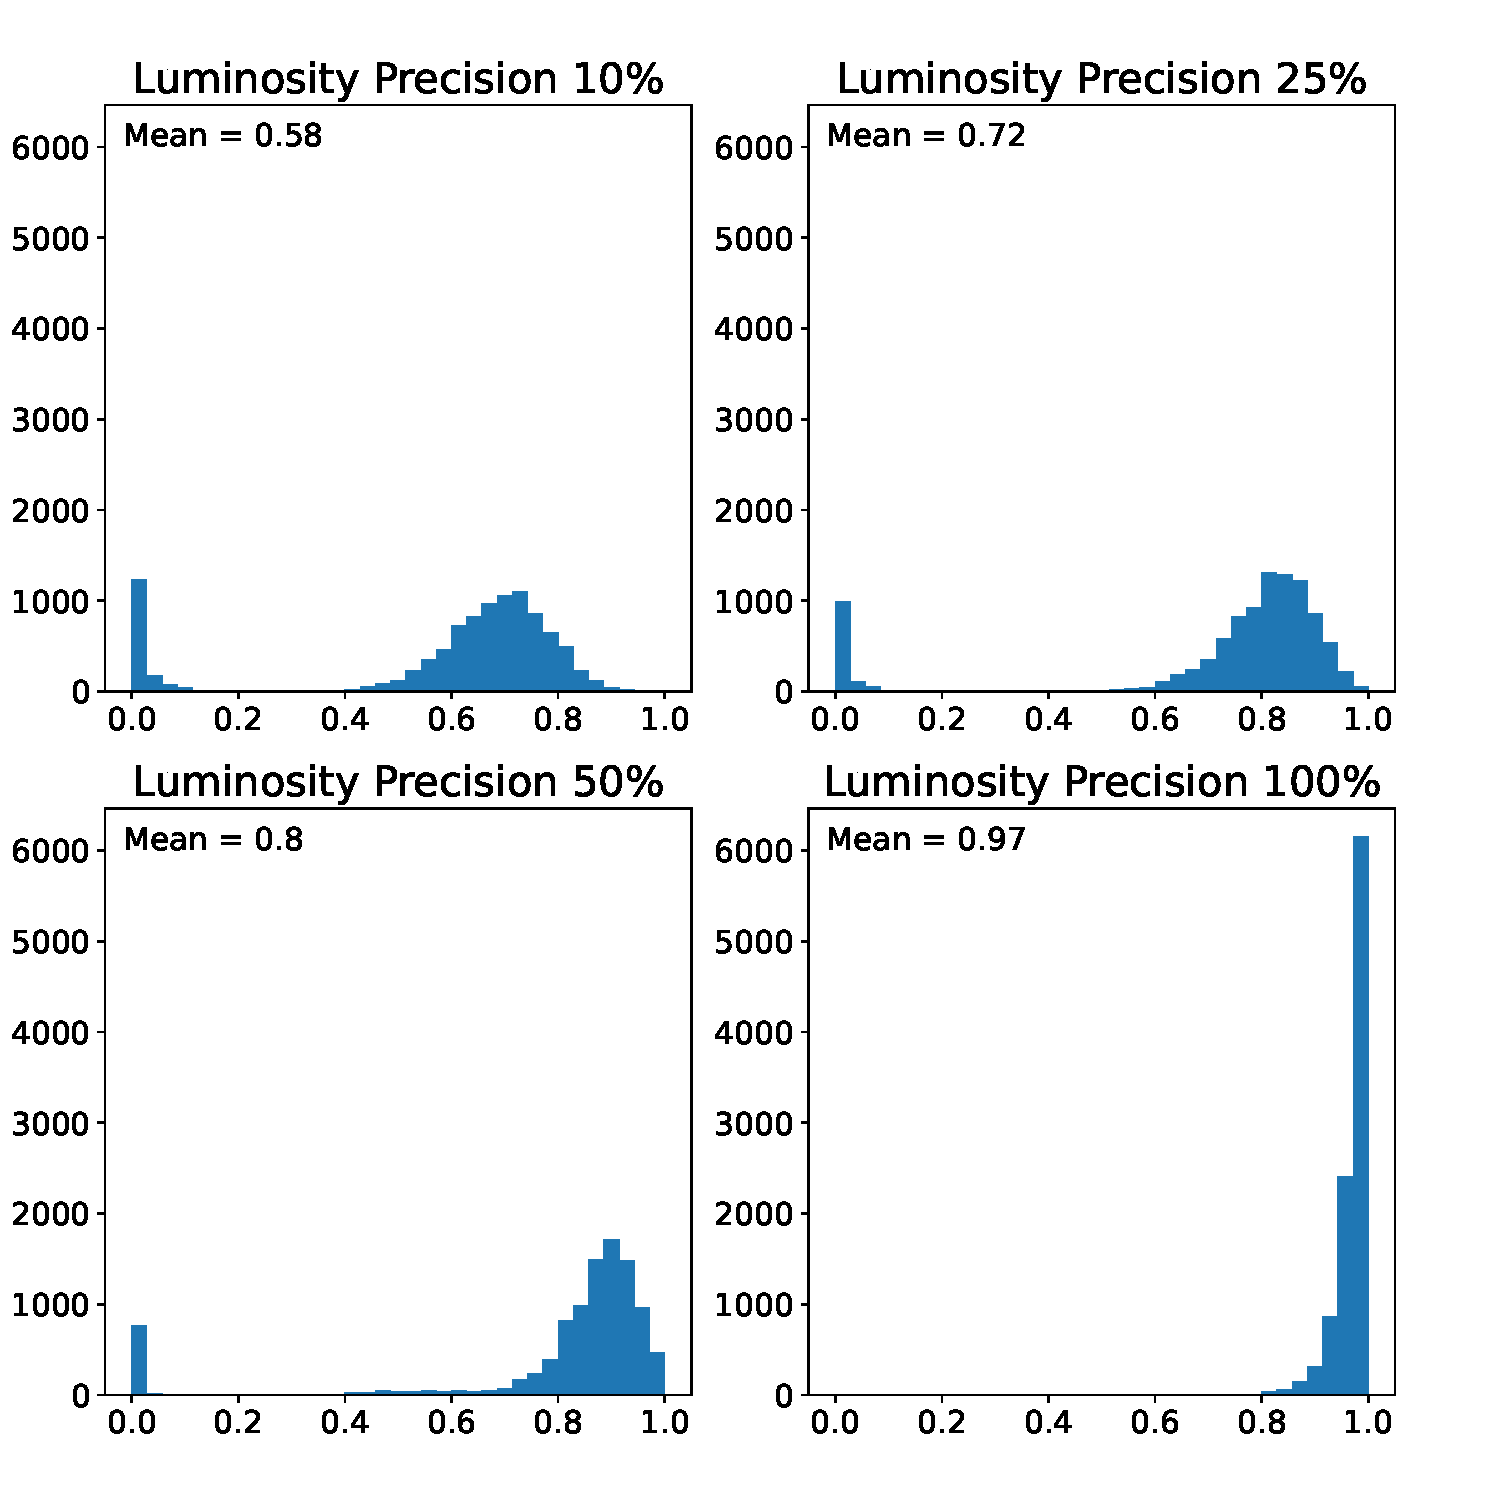
\includegraphics[height=0.4\textheight]{backgauss2_hists_lucy.pdf}
			\caption{Completeness distribution of RL reconstruction, $\sigma = 2$, off = 10}
			\label{fig:bhl}
		\end{figure}
		\newpage
		\null
		\vfill
		\begin{figure}[h]
			\centering
			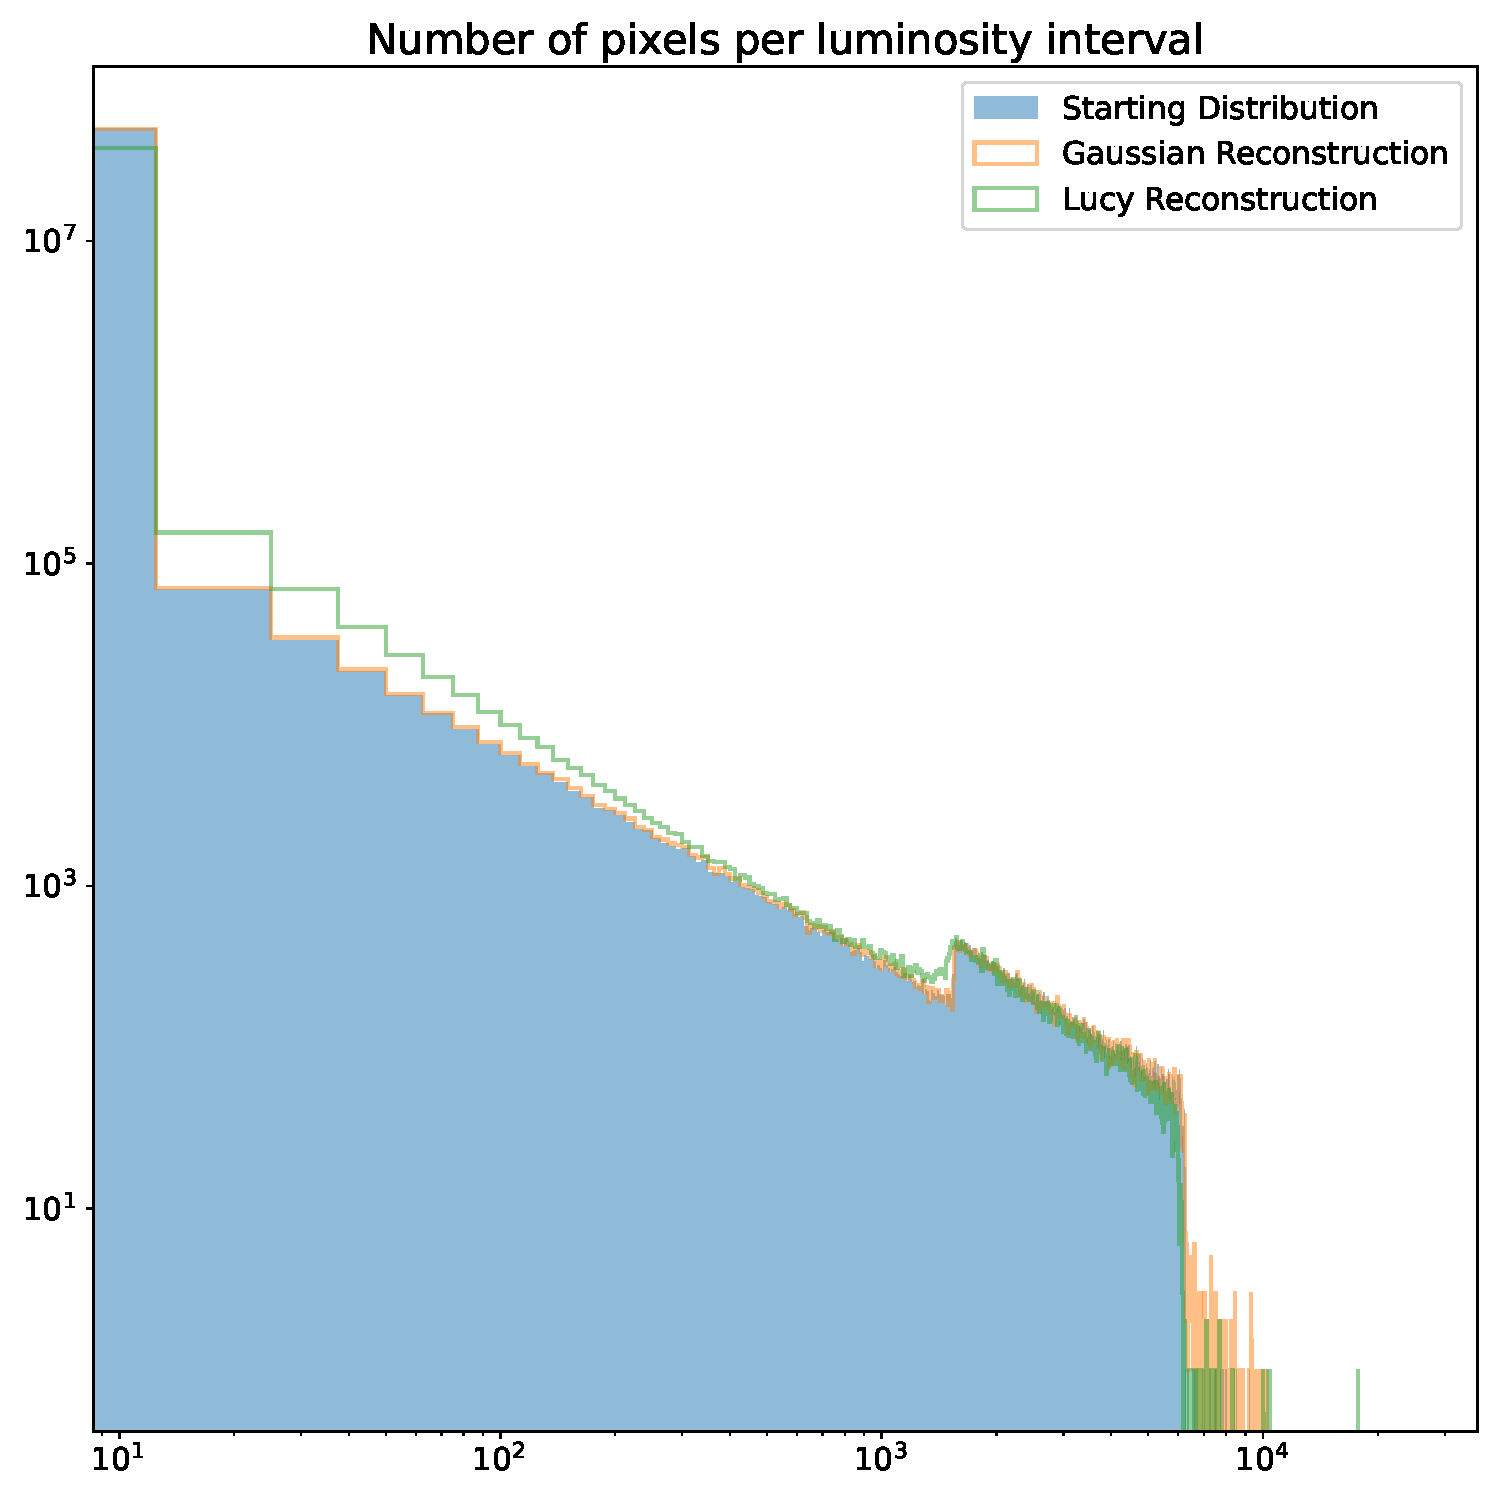
\includegraphics[height=0.4\textheight]{backgauss2_lumin.pdf}
			\caption{Luminosity distribution, $\sigma = 2$, off = 10}
			\label{fig:bl}
		\end{figure}
		\vfill
		\newpage
		\begin{figure}[h!]
			\centering
			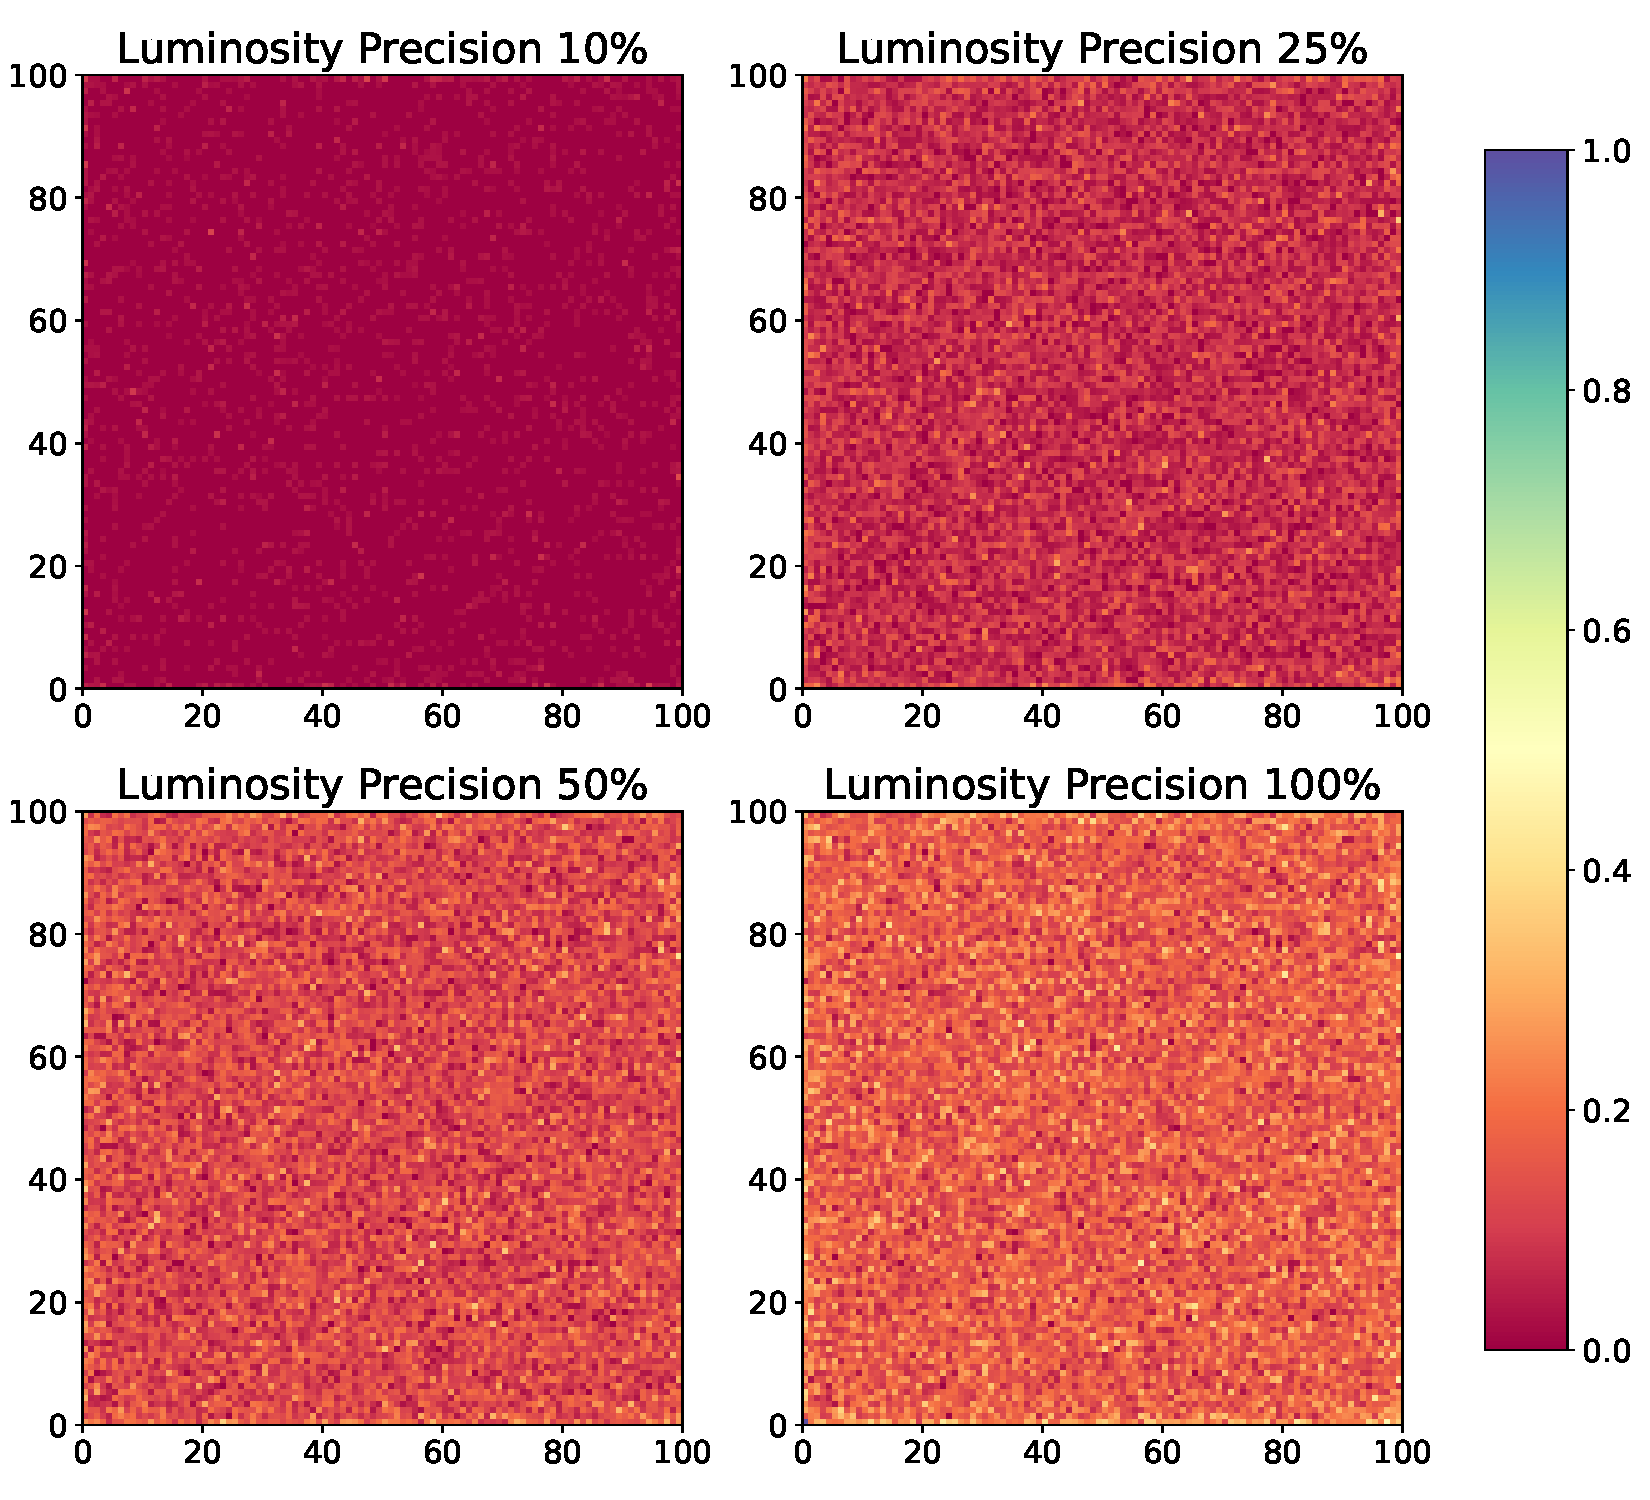
\includegraphics[height=0.4\textheight]{poissgauss2_boards_gauss.pdf}
			\caption{Completeness of Gaussian fit, $\sigma = 2$, off = 0, Poisson noise}
			\label{fig:pbg}
		\end{figure}
		\begin{figure}[h!]
			\centering
			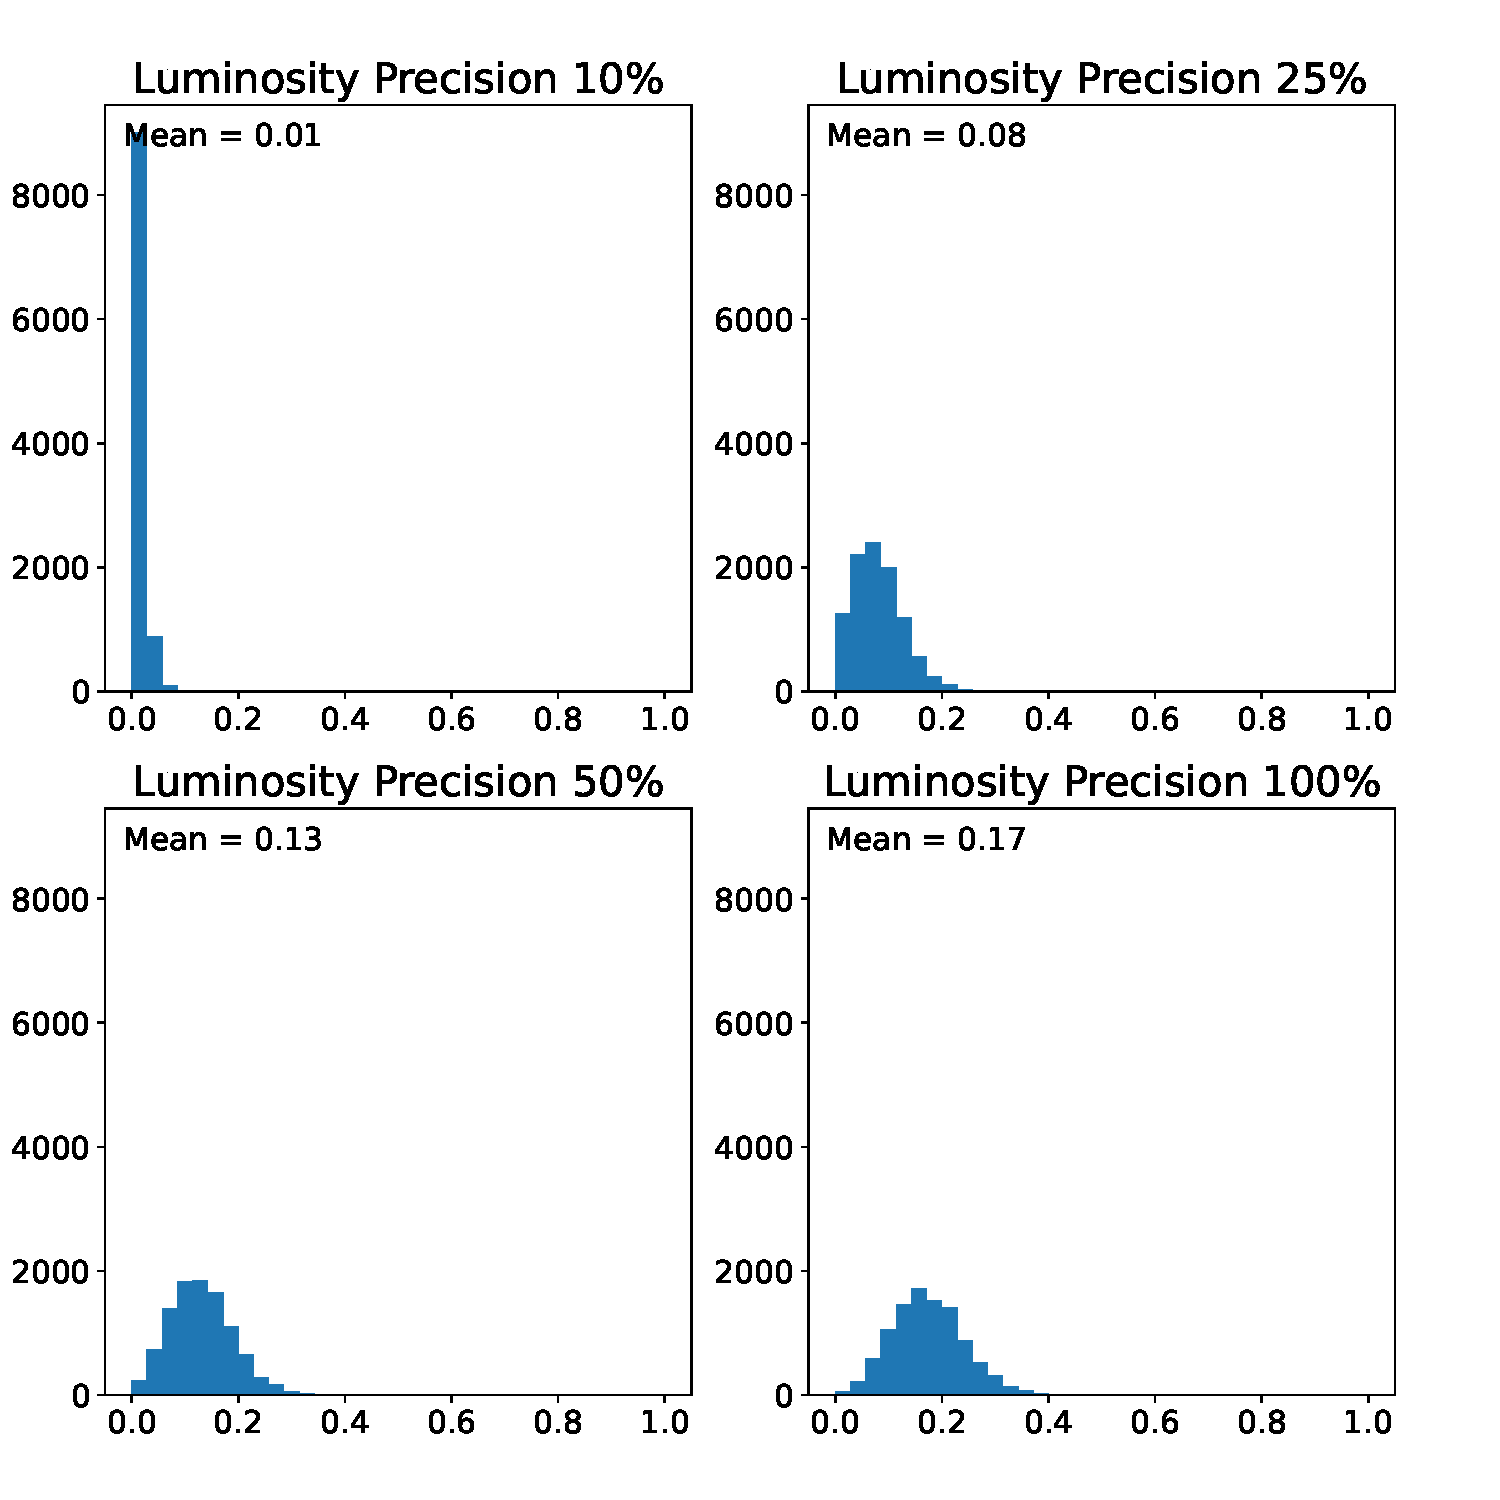
\includegraphics[height=0.4\textheight]{poissgauss2_hists_gauss.pdf}
			\caption{Completeness distribution of Gaussian fit, $\sigma = 2$, off = 0, Poisson noise}
			\label{fig:phg}
		\end{figure}
		\newpage
		\begin{figure}[h!]
			\centering
			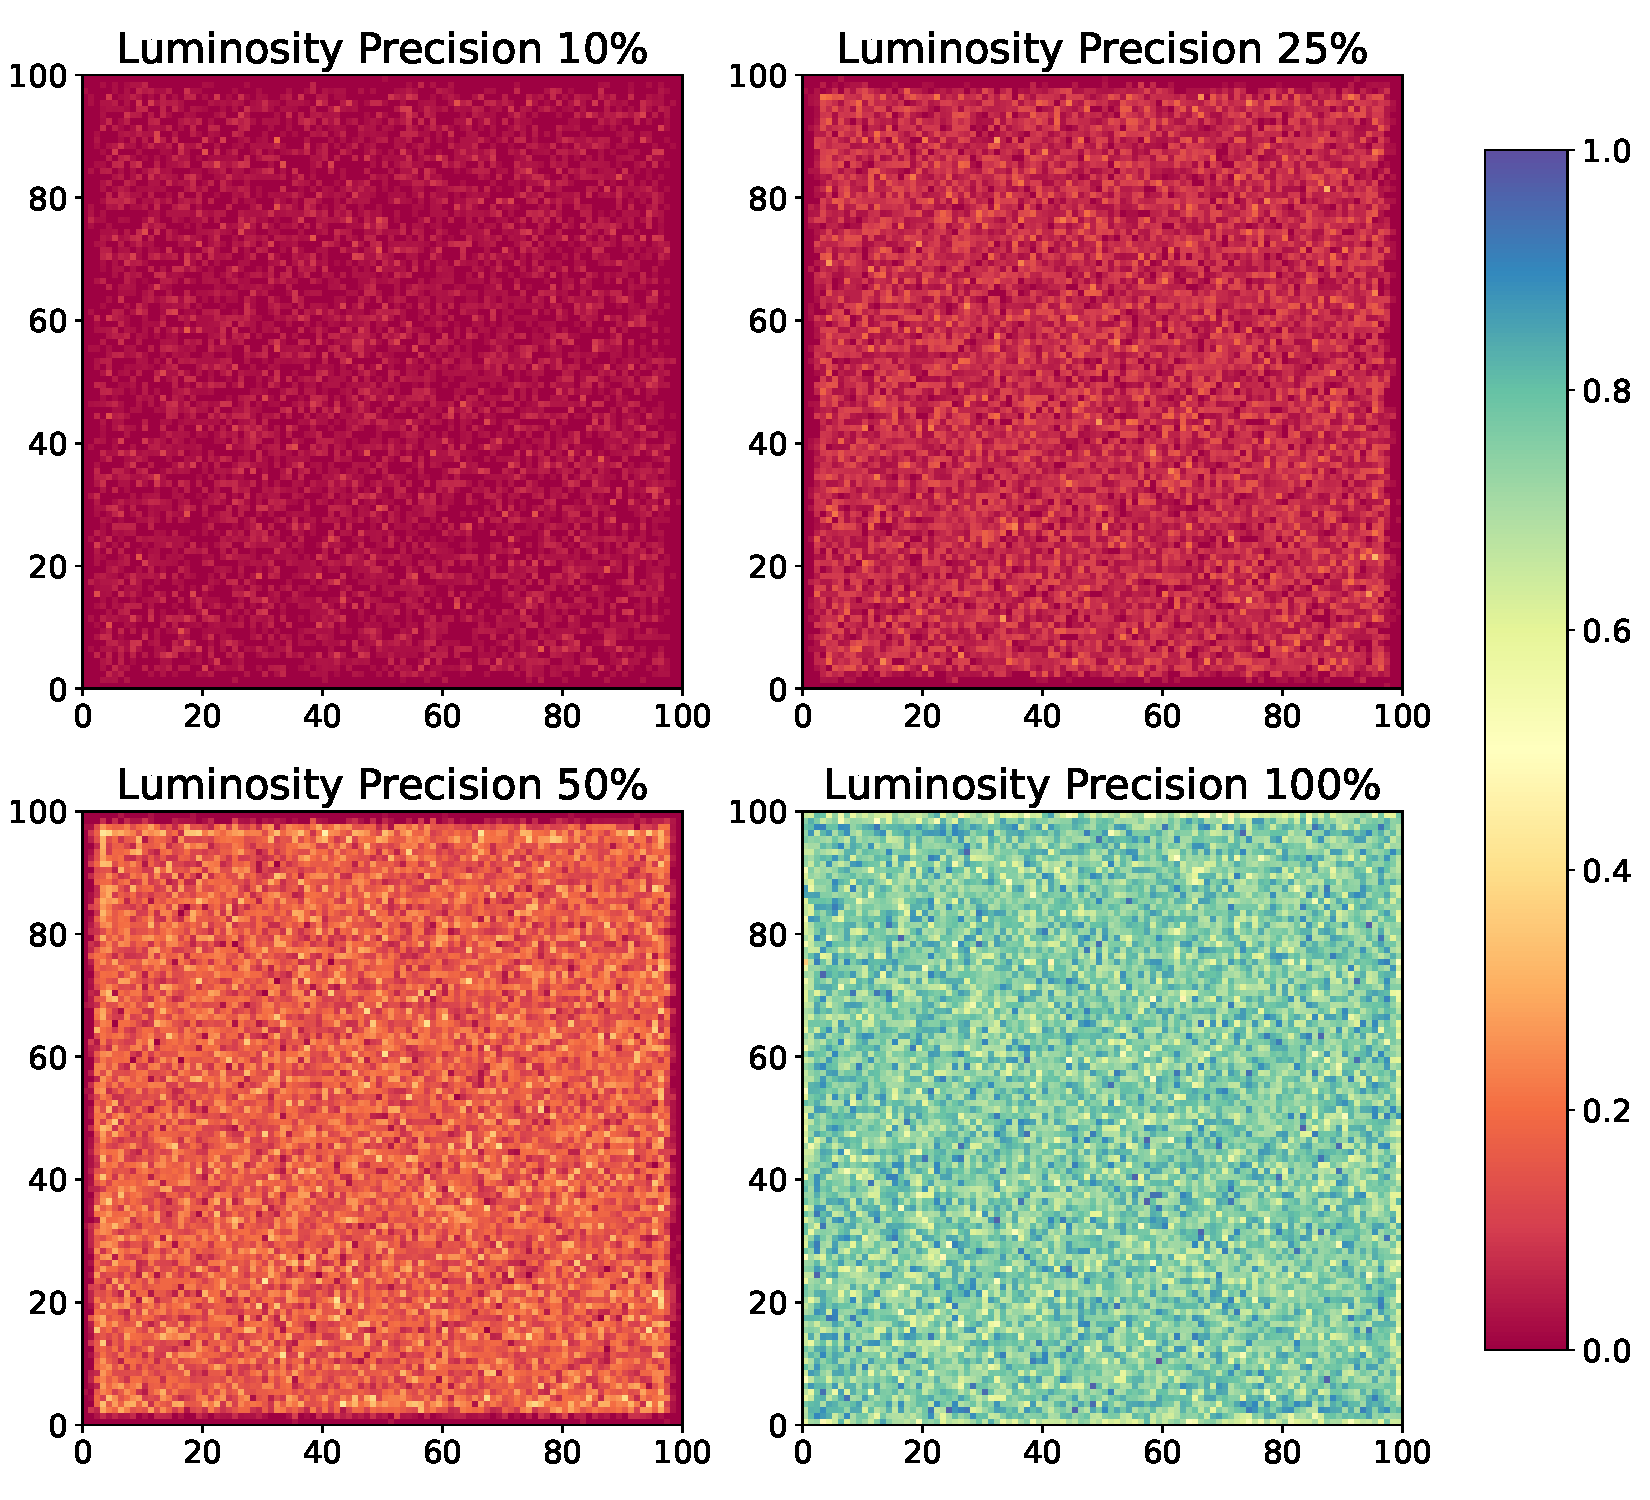
\includegraphics[height=0.4\textheight]{poissgauss2_boards_lucy.pdf}
			\caption{Completeness of RL reconstruction, $\sigma = 2$, off = 0, Poisson noise}
			\label{fig:pbl}
		\end{figure}
		\begin{figure}[h!]
			\centering
			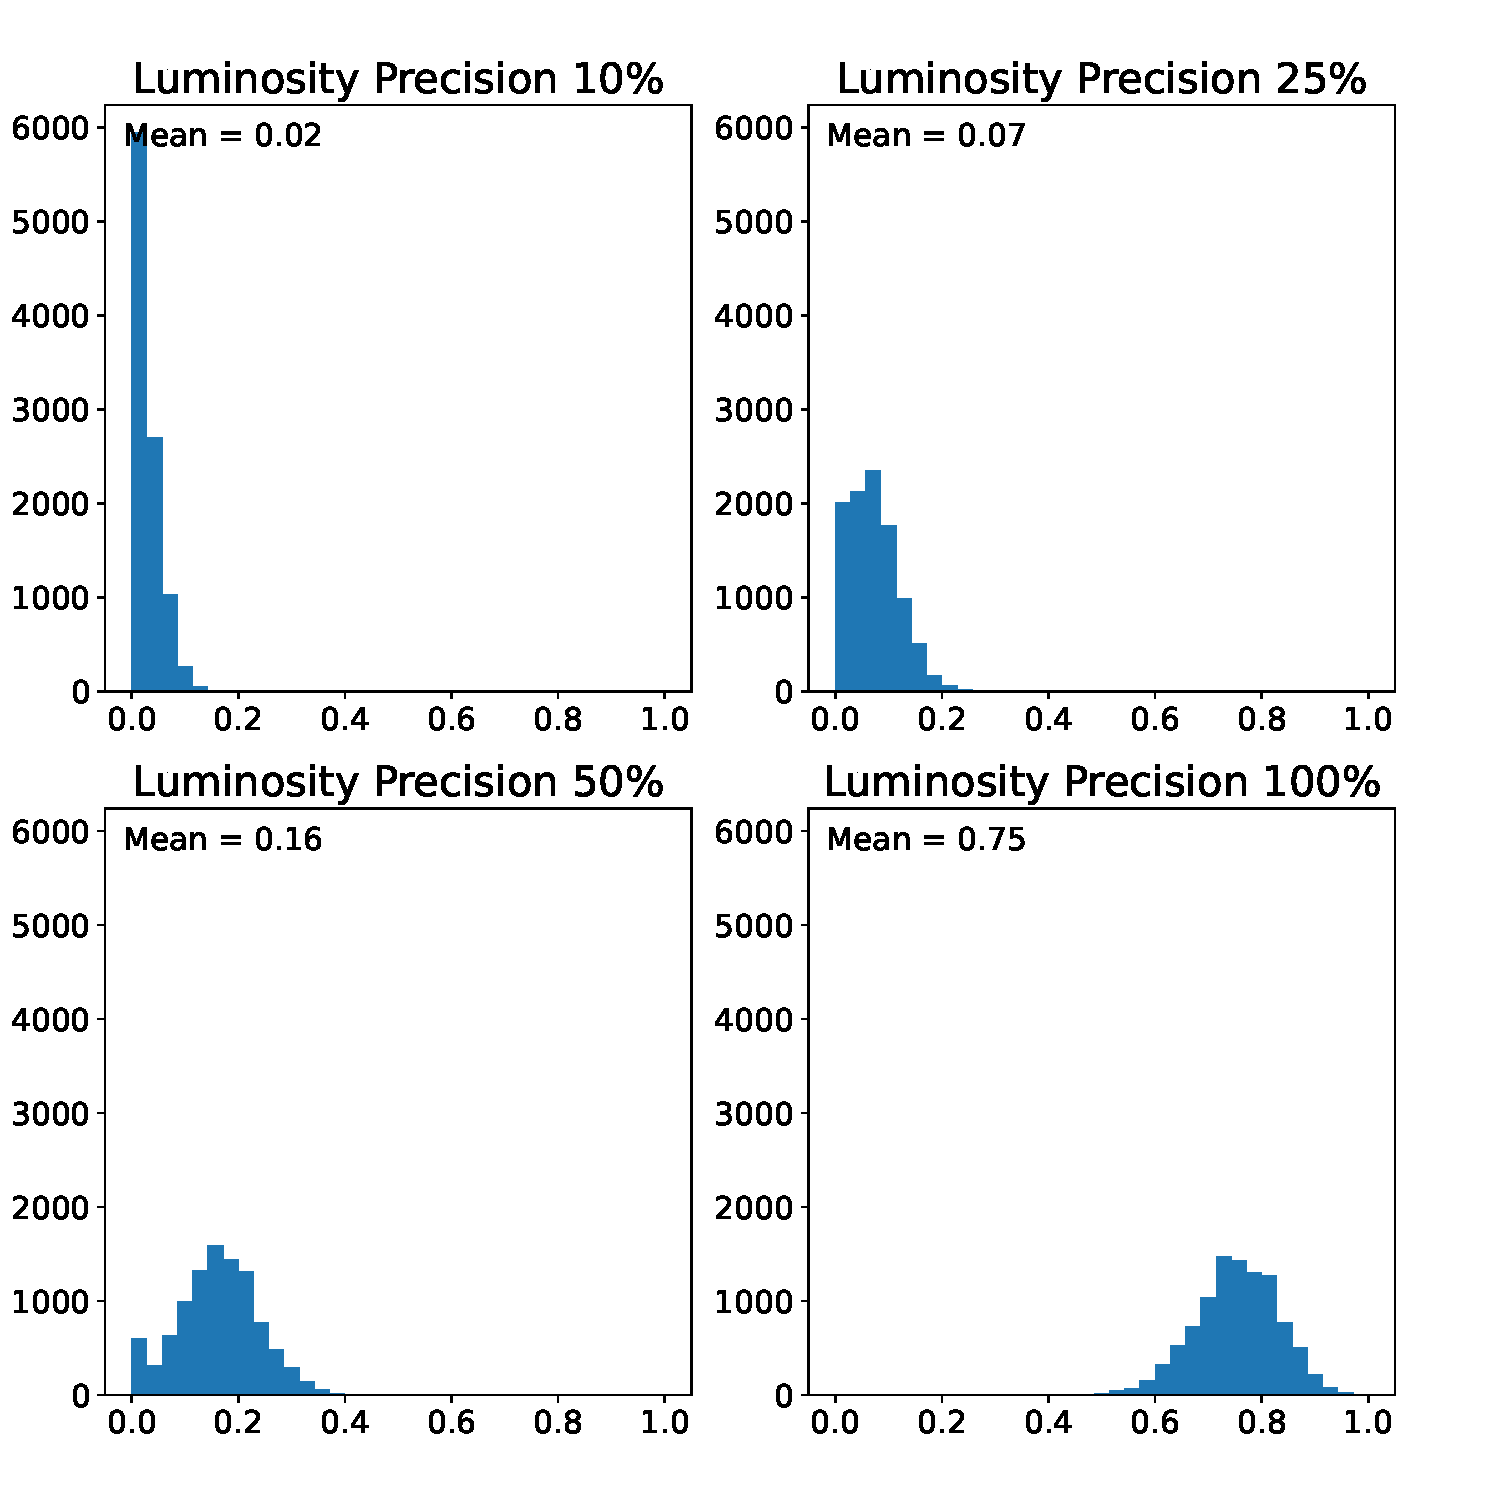
\includegraphics[height=0.4\textheight]{poissgauss2_hists_lucy.pdf}
			\caption{Completeness distribution of RL reconstruction, $\sigma = 2$, off = 0, Poisson noise}
			\label{fig:phl}
		\end{figure}
		\newpage
		\null
		\vfill
		\begin{figure}[h]
			\centering
			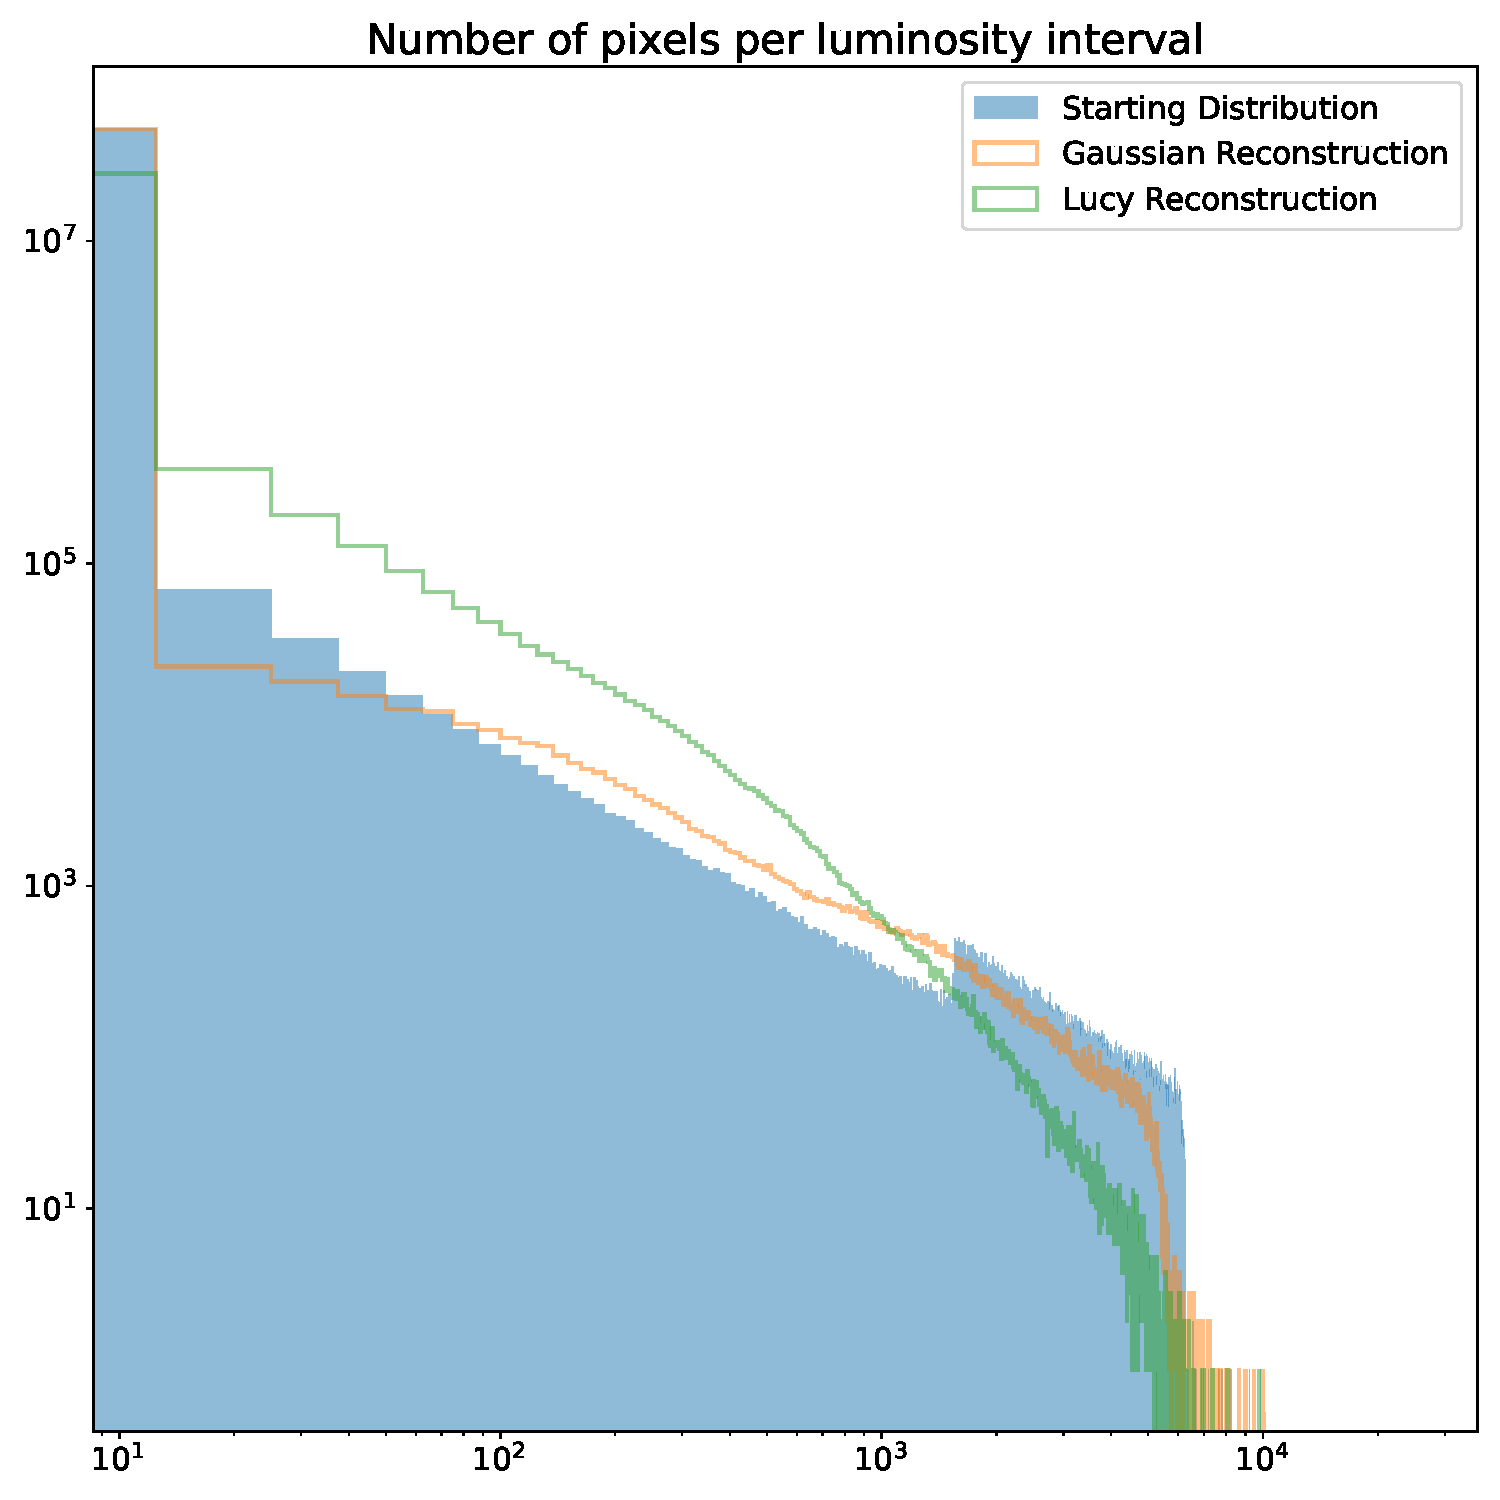
\includegraphics[height=0.4\textheight]{poissgauss2_lumin.pdf}
			\caption{Luminosity distribution, $\sigma = 2$, off = 0, Poisson noise}
			\label{fig:pl}
		\end{figure}
		\vfill
	
\end{document}